\begin{figure}[H] \centering % Created by tikzDevice version 0.12.4 on 2023-07-18 17:44:28
% !TEX encoding = UTF-8 Unicode
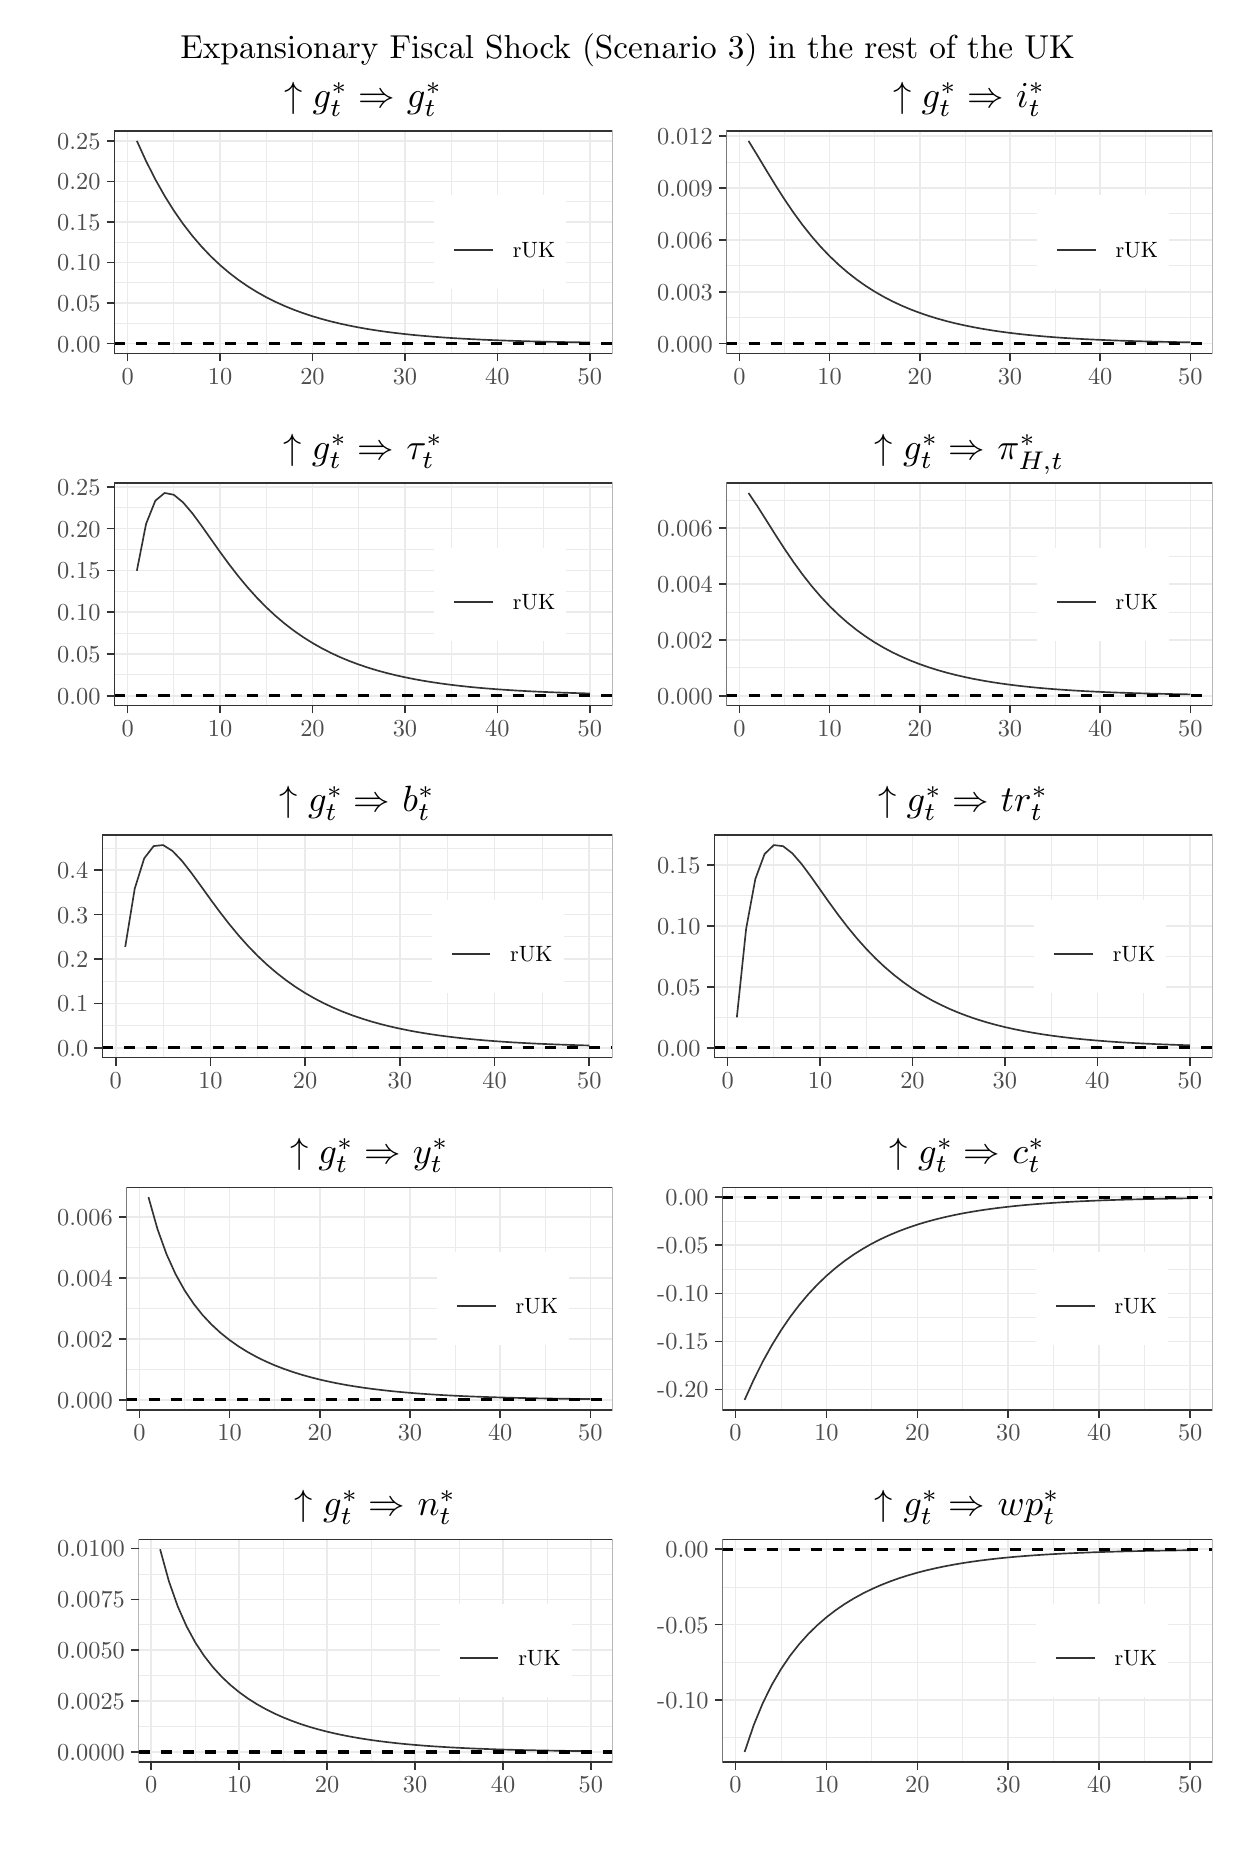
\begin{tikzpicture}[x=1pt,y=1pt]
\definecolor{fillColor}{RGB}{255,255,255}
\path[use as bounding box,fill=fillColor,fill opacity=0.00] (0,0) rectangle (433.62,650.43);
\begin{scope}
\path[clip] (  0.00,508.91) rectangle (216.81,636.14);
\definecolor{drawColor}{RGB}{255,255,255}
\definecolor{fillColor}{RGB}{255,255,255}

\path[draw=drawColor,line width= 0.6pt,line join=round,line cap=round,fill=fillColor] (  0.00,508.91) rectangle (216.81,636.14);
\end{scope}
\begin{scope}
\path[clip] ( 31.27,532.59) rectangle (211.31,613.18);
\definecolor{fillColor}{RGB}{255,255,255}

\path[fill=fillColor] ( 31.27,532.59) rectangle (211.31,613.18);
\definecolor{drawColor}{gray}{0.92}

\path[draw=drawColor,line width= 0.3pt,line join=round] ( 31.27,543.58) --
	(211.31,543.58);

\path[draw=drawColor,line width= 0.3pt,line join=round] ( 31.27,558.23) --
	(211.31,558.23);

\path[draw=drawColor,line width= 0.3pt,line join=round] ( 31.27,572.89) --
	(211.31,572.89);

\path[draw=drawColor,line width= 0.3pt,line join=round] ( 31.27,587.54) --
	(211.31,587.54);

\path[draw=drawColor,line width= 0.3pt,line join=round] ( 31.27,602.19) --
	(211.31,602.19);

\path[draw=drawColor,line width= 0.3pt,line join=round] ( 52.81,532.59) --
	( 52.81,613.18);

\path[draw=drawColor,line width= 0.3pt,line join=round] ( 86.22,532.59) --
	( 86.22,613.18);

\path[draw=drawColor,line width= 0.3pt,line join=round] (119.62,532.59) --
	(119.62,613.18);

\path[draw=drawColor,line width= 0.3pt,line join=round] (153.02,532.59) --
	(153.02,613.18);

\path[draw=drawColor,line width= 0.3pt,line join=round] (186.43,532.59) --
	(186.43,613.18);

\path[draw=drawColor,line width= 0.6pt,line join=round] ( 31.27,536.25) --
	(211.31,536.25);

\path[draw=drawColor,line width= 0.6pt,line join=round] ( 31.27,550.91) --
	(211.31,550.91);

\path[draw=drawColor,line width= 0.6pt,line join=round] ( 31.27,565.56) --
	(211.31,565.56);

\path[draw=drawColor,line width= 0.6pt,line join=round] ( 31.27,580.21) --
	(211.31,580.21);

\path[draw=drawColor,line width= 0.6pt,line join=round] ( 31.27,594.87) --
	(211.31,594.87);

\path[draw=drawColor,line width= 0.6pt,line join=round] ( 31.27,609.52) --
	(211.31,609.52);

\path[draw=drawColor,line width= 0.6pt,line join=round] ( 36.11,532.59) --
	( 36.11,613.18);

\path[draw=drawColor,line width= 0.6pt,line join=round] ( 69.52,532.59) --
	( 69.52,613.18);

\path[draw=drawColor,line width= 0.6pt,line join=round] (102.92,532.59) --
	(102.92,613.18);

\path[draw=drawColor,line width= 0.6pt,line join=round] (136.32,532.59) --
	(136.32,613.18);

\path[draw=drawColor,line width= 0.6pt,line join=round] (169.72,532.59) --
	(169.72,613.18);

\path[draw=drawColor,line width= 0.6pt,line join=round] (203.13,532.59) --
	(203.13,613.18);
\definecolor{drawColor}{gray}{0.20}

\path[draw=drawColor,line width= 0.6pt,line join=round] ( 39.45,609.52) --
	( 42.79,602.19) --
	( 46.13,595.60) --
	( 49.47,589.66) --
	( 52.81,584.32) --
	( 56.15,579.52) --
	( 59.50,575.19) --
	( 62.84,571.30) --
	( 66.18,567.79) --
	( 69.52,564.64) --
	( 72.86,561.80) --
	( 76.20,559.25) --
	( 79.54,556.95) --
	( 82.88,554.88) --
	( 86.22,553.01) --
	( 89.56,551.34) --
	( 92.90,549.83) --
	( 96.24,548.47) --
	( 99.58,547.25) --
	(102.92,546.15) --
	(106.26,545.16) --
	(109.60,544.27) --
	(112.94,543.47) --
	(116.28,542.75) --
	(119.62,542.10) --
	(122.96,541.51) --
	(126.30,540.99) --
	(129.64,540.51) --
	(132.98,540.09) --
	(136.32,539.71) --
	(139.66,539.36) --
	(143.00,539.05) --
	(146.34,538.77) --
	(149.68,538.52) --
	(153.02,538.29) --
	(156.36,538.09) --
	(159.70,537.91) --
	(163.04,537.74) --
	(166.38,537.59) --
	(169.72,537.46) --
	(173.06,537.34) --
	(176.40,537.23) --
	(179.74,537.13) --
	(183.08,537.04) --
	(186.43,536.97) --
	(189.77,536.89) --
	(193.11,536.83) --
	(196.45,536.77) --
	(199.79,536.72) --
	(203.13,536.67);
\definecolor{drawColor}{RGB}{0,0,0}

\path[draw=drawColor,line width= 1.1pt,dash pattern=on 4pt off 4pt ,line join=round] ( 31.27,536.25) -- (211.31,536.25);
\definecolor{drawColor}{gray}{0.20}

\path[draw=drawColor,line width= 0.6pt,line join=round,line cap=round] ( 31.27,532.59) rectangle (211.31,613.18);
\end{scope}
\begin{scope}
\path[clip] (  0.00,  0.00) rectangle (433.62,650.43);
\definecolor{drawColor}{gray}{0.30}

\node[text=drawColor,anchor=base east,inner sep=0pt, outer sep=0pt, scale=  0.88] at ( 26.32,533.22) {0.00};

\node[text=drawColor,anchor=base east,inner sep=0pt, outer sep=0pt, scale=  0.88] at ( 26.32,547.88) {0.05};

\node[text=drawColor,anchor=base east,inner sep=0pt, outer sep=0pt, scale=  0.88] at ( 26.32,562.53) {0.10};

\node[text=drawColor,anchor=base east,inner sep=0pt, outer sep=0pt, scale=  0.88] at ( 26.32,577.18) {0.15};

\node[text=drawColor,anchor=base east,inner sep=0pt, outer sep=0pt, scale=  0.88] at ( 26.32,591.83) {0.20};

\node[text=drawColor,anchor=base east,inner sep=0pt, outer sep=0pt, scale=  0.88] at ( 26.32,606.49) {0.25};
\end{scope}
\begin{scope}
\path[clip] (  0.00,  0.00) rectangle (433.62,650.43);
\definecolor{drawColor}{gray}{0.20}

\path[draw=drawColor,line width= 0.6pt,line join=round] ( 28.52,536.25) --
	( 31.27,536.25);

\path[draw=drawColor,line width= 0.6pt,line join=round] ( 28.52,550.91) --
	( 31.27,550.91);

\path[draw=drawColor,line width= 0.6pt,line join=round] ( 28.52,565.56) --
	( 31.27,565.56);

\path[draw=drawColor,line width= 0.6pt,line join=round] ( 28.52,580.21) --
	( 31.27,580.21);

\path[draw=drawColor,line width= 0.6pt,line join=round] ( 28.52,594.87) --
	( 31.27,594.87);

\path[draw=drawColor,line width= 0.6pt,line join=round] ( 28.52,609.52) --
	( 31.27,609.52);
\end{scope}
\begin{scope}
\path[clip] (  0.00,  0.00) rectangle (433.62,650.43);
\definecolor{drawColor}{gray}{0.20}

\path[draw=drawColor,line width= 0.6pt,line join=round] ( 36.11,529.84) --
	( 36.11,532.59);

\path[draw=drawColor,line width= 0.6pt,line join=round] ( 69.52,529.84) --
	( 69.52,532.59);

\path[draw=drawColor,line width= 0.6pt,line join=round] (102.92,529.84) --
	(102.92,532.59);

\path[draw=drawColor,line width= 0.6pt,line join=round] (136.32,529.84) --
	(136.32,532.59);

\path[draw=drawColor,line width= 0.6pt,line join=round] (169.72,529.84) --
	(169.72,532.59);

\path[draw=drawColor,line width= 0.6pt,line join=round] (203.13,529.84) --
	(203.13,532.59);
\end{scope}
\begin{scope}
\path[clip] (  0.00,  0.00) rectangle (433.62,650.43);
\definecolor{drawColor}{gray}{0.30}

\node[text=drawColor,anchor=base,inner sep=0pt, outer sep=0pt, scale=  0.88] at ( 36.11,521.58) {0};

\node[text=drawColor,anchor=base,inner sep=0pt, outer sep=0pt, scale=  0.88] at ( 69.52,521.58) {10};

\node[text=drawColor,anchor=base,inner sep=0pt, outer sep=0pt, scale=  0.88] at (102.92,521.58) {20};

\node[text=drawColor,anchor=base,inner sep=0pt, outer sep=0pt, scale=  0.88] at (136.32,521.58) {30};

\node[text=drawColor,anchor=base,inner sep=0pt, outer sep=0pt, scale=  0.88] at (169.72,521.58) {40};

\node[text=drawColor,anchor=base,inner sep=0pt, outer sep=0pt, scale=  0.88] at (203.13,521.58) {50};
\end{scope}
\begin{scope}
\path[clip] (  0.00,  0.00) rectangle (433.62,650.43);
\definecolor{fillColor}{RGB}{255,255,255}

\path[fill=fillColor] (146.96,555.96) rectangle (194.64,589.81);
\end{scope}
\begin{scope}
\path[clip] (  0.00,  0.00) rectangle (433.62,650.43);
\definecolor{fillColor}{RGB}{255,255,255}

\path[fill=fillColor] (152.46,561.46) rectangle (169.81,578.81);
\end{scope}
\begin{scope}
\path[clip] (  0.00,  0.00) rectangle (433.62,650.43);
\definecolor{drawColor}{gray}{0.20}

\path[draw=drawColor,line width= 0.6pt,line join=round] (154.20,570.14) -- (168.08,570.14);
\end{scope}
\begin{scope}
\path[clip] (  0.00,  0.00) rectangle (433.62,650.43);
\definecolor{drawColor}{RGB}{0,0,0}

\node[text=drawColor,anchor=base west,inner sep=0pt, outer sep=0pt, scale=  0.80] at (175.31,567.38) {rUK};
\end{scope}
\begin{scope}
\path[clip] (  0.00,  0.00) rectangle (433.62,650.43);
\definecolor{drawColor}{RGB}{0,0,0}

\node[text=drawColor,anchor=base,inner sep=0pt, outer sep=0pt, scale=  1.32] at (121.29,621.55) {$\uparrow  g^*_t \Rightarrow $ ${g^*_t}$};
\end{scope}
\begin{scope}
\path[clip] (216.81,508.91) rectangle (433.62,636.14);
\definecolor{drawColor}{RGB}{255,255,255}
\definecolor{fillColor}{RGB}{255,255,255}

\path[draw=drawColor,line width= 0.6pt,line join=round,line cap=round,fill=fillColor] (216.81,508.91) rectangle (433.62,636.14);
\end{scope}
\begin{scope}
\path[clip] (252.48,532.59) rectangle (428.12,613.18);
\definecolor{fillColor}{RGB}{255,255,255}

\path[fill=fillColor] (252.48,532.59) rectangle (428.12,613.18);
\definecolor{drawColor}{gray}{0.92}

\path[draw=drawColor,line width= 0.3pt,line join=round] (252.48,545.63) --
	(428.12,545.63);

\path[draw=drawColor,line width= 0.3pt,line join=round] (252.48,564.38) --
	(428.12,564.38);

\path[draw=drawColor,line width= 0.3pt,line join=round] (252.48,583.13) --
	(428.12,583.13);

\path[draw=drawColor,line width= 0.3pt,line join=round] (252.48,601.88) --
	(428.12,601.88);

\path[draw=drawColor,line width= 0.3pt,line join=round] (273.50,532.59) --
	(273.50,613.18);

\path[draw=drawColor,line width= 0.3pt,line join=round] (306.08,532.59) --
	(306.08,613.18);

\path[draw=drawColor,line width= 0.3pt,line join=round] (338.67,532.59) --
	(338.67,613.18);

\path[draw=drawColor,line width= 0.3pt,line join=round] (371.26,532.59) --
	(371.26,613.18);

\path[draw=drawColor,line width= 0.3pt,line join=round] (403.84,532.59) --
	(403.84,613.18);

\path[draw=drawColor,line width= 0.6pt,line join=round] (252.48,536.25) --
	(428.12,536.25);

\path[draw=drawColor,line width= 0.6pt,line join=round] (252.48,555.00) --
	(428.12,555.00);

\path[draw=drawColor,line width= 0.6pt,line join=round] (252.48,573.76) --
	(428.12,573.76);

\path[draw=drawColor,line width= 0.6pt,line join=round] (252.48,592.51) --
	(428.12,592.51);

\path[draw=drawColor,line width= 0.6pt,line join=round] (252.48,611.26) --
	(428.12,611.26);

\path[draw=drawColor,line width= 0.6pt,line join=round] (257.20,532.59) --
	(257.20,613.18);

\path[draw=drawColor,line width= 0.6pt,line join=round] (289.79,532.59) --
	(289.79,613.18);

\path[draw=drawColor,line width= 0.6pt,line join=round] (322.38,532.59) --
	(322.38,613.18);

\path[draw=drawColor,line width= 0.6pt,line join=round] (354.96,532.59) --
	(354.96,613.18);

\path[draw=drawColor,line width= 0.6pt,line join=round] (387.55,532.59) --
	(387.55,613.18);

\path[draw=drawColor,line width= 0.6pt,line join=round] (420.14,532.59) --
	(420.14,613.18);
\definecolor{drawColor}{gray}{0.20}

\path[draw=drawColor,line width= 0.6pt,line join=round] (260.46,609.52) --
	(263.72,604.20) --
	(266.98,598.77) --
	(270.24,593.44) --
	(273.50,588.34) --
	(276.76,583.55) --
	(280.01,579.11) --
	(283.27,575.02) --
	(286.53,571.27) --
	(289.79,567.86) --
	(293.05,564.76) --
	(296.31,561.95) --
	(299.57,559.41) --
	(302.82,557.11) --
	(306.08,555.04) --
	(309.34,553.17) --
	(312.60,551.48) --
	(315.86,549.96) --
	(319.12,548.59) --
	(322.38,547.36) --
	(325.64,546.25) --
	(328.89,545.25) --
	(332.15,544.35) --
	(335.41,543.54) --
	(338.67,542.82) --
	(341.93,542.16) --
	(345.19,541.57) --
	(348.45,541.04) --
	(351.70,540.56) --
	(354.96,540.13) --
	(358.22,539.74) --
	(361.48,539.39) --
	(364.74,539.08) --
	(368.00,538.80) --
	(371.26,538.54) --
	(374.52,538.31) --
	(377.77,538.11) --
	(381.03,537.92) --
	(384.29,537.76) --
	(387.55,537.61) --
	(390.81,537.47) --
	(394.07,537.35) --
	(397.33,537.24) --
	(400.58,537.14) --
	(403.84,537.05) --
	(407.10,536.97) --
	(410.36,536.90) --
	(413.62,536.84) --
	(416.88,536.78) --
	(420.14,536.73);
\definecolor{drawColor}{RGB}{0,0,0}

\path[draw=drawColor,line width= 1.1pt,dash pattern=on 4pt off 4pt ,line join=round] (252.48,536.25) -- (428.12,536.25);
\definecolor{drawColor}{gray}{0.20}

\path[draw=drawColor,line width= 0.6pt,line join=round,line cap=round] (252.48,532.59) rectangle (428.12,613.18);
\end{scope}
\begin{scope}
\path[clip] (  0.00,  0.00) rectangle (433.62,650.43);
\definecolor{drawColor}{gray}{0.30}

\node[text=drawColor,anchor=base east,inner sep=0pt, outer sep=0pt, scale=  0.88] at (247.53,533.22) {0.000};

\node[text=drawColor,anchor=base east,inner sep=0pt, outer sep=0pt, scale=  0.88] at (247.53,551.97) {0.003};

\node[text=drawColor,anchor=base east,inner sep=0pt, outer sep=0pt, scale=  0.88] at (247.53,570.72) {0.006};

\node[text=drawColor,anchor=base east,inner sep=0pt, outer sep=0pt, scale=  0.88] at (247.53,589.47) {0.009};

\node[text=drawColor,anchor=base east,inner sep=0pt, outer sep=0pt, scale=  0.88] at (247.53,608.22) {0.012};
\end{scope}
\begin{scope}
\path[clip] (  0.00,  0.00) rectangle (433.62,650.43);
\definecolor{drawColor}{gray}{0.20}

\path[draw=drawColor,line width= 0.6pt,line join=round] (249.73,536.25) --
	(252.48,536.25);

\path[draw=drawColor,line width= 0.6pt,line join=round] (249.73,555.00) --
	(252.48,555.00);

\path[draw=drawColor,line width= 0.6pt,line join=round] (249.73,573.76) --
	(252.48,573.76);

\path[draw=drawColor,line width= 0.6pt,line join=round] (249.73,592.51) --
	(252.48,592.51);

\path[draw=drawColor,line width= 0.6pt,line join=round] (249.73,611.26) --
	(252.48,611.26);
\end{scope}
\begin{scope}
\path[clip] (  0.00,  0.00) rectangle (433.62,650.43);
\definecolor{drawColor}{gray}{0.20}

\path[draw=drawColor,line width= 0.6pt,line join=round] (257.20,529.84) --
	(257.20,532.59);

\path[draw=drawColor,line width= 0.6pt,line join=round] (289.79,529.84) --
	(289.79,532.59);

\path[draw=drawColor,line width= 0.6pt,line join=round] (322.38,529.84) --
	(322.38,532.59);

\path[draw=drawColor,line width= 0.6pt,line join=round] (354.96,529.84) --
	(354.96,532.59);

\path[draw=drawColor,line width= 0.6pt,line join=round] (387.55,529.84) --
	(387.55,532.59);

\path[draw=drawColor,line width= 0.6pt,line join=round] (420.14,529.84) --
	(420.14,532.59);
\end{scope}
\begin{scope}
\path[clip] (  0.00,  0.00) rectangle (433.62,650.43);
\definecolor{drawColor}{gray}{0.30}

\node[text=drawColor,anchor=base,inner sep=0pt, outer sep=0pt, scale=  0.88] at (257.20,521.58) {0};

\node[text=drawColor,anchor=base,inner sep=0pt, outer sep=0pt, scale=  0.88] at (289.79,521.58) {10};

\node[text=drawColor,anchor=base,inner sep=0pt, outer sep=0pt, scale=  0.88] at (322.38,521.58) {20};

\node[text=drawColor,anchor=base,inner sep=0pt, outer sep=0pt, scale=  0.88] at (354.96,521.58) {30};

\node[text=drawColor,anchor=base,inner sep=0pt, outer sep=0pt, scale=  0.88] at (387.55,521.58) {40};

\node[text=drawColor,anchor=base,inner sep=0pt, outer sep=0pt, scale=  0.88] at (420.14,521.58) {50};
\end{scope}
\begin{scope}
\path[clip] (  0.00,  0.00) rectangle (433.62,650.43);
\definecolor{fillColor}{RGB}{255,255,255}

\path[fill=fillColor] (364.76,555.96) rectangle (412.44,589.81);
\end{scope}
\begin{scope}
\path[clip] (  0.00,  0.00) rectangle (433.62,650.43);
\definecolor{fillColor}{RGB}{255,255,255}

\path[fill=fillColor] (370.26,561.46) rectangle (387.61,578.81);
\end{scope}
\begin{scope}
\path[clip] (  0.00,  0.00) rectangle (433.62,650.43);
\definecolor{drawColor}{gray}{0.20}

\path[draw=drawColor,line width= 0.6pt,line join=round] (372.00,570.14) -- (385.87,570.14);
\end{scope}
\begin{scope}
\path[clip] (  0.00,  0.00) rectangle (433.62,650.43);
\definecolor{drawColor}{RGB}{0,0,0}

\node[text=drawColor,anchor=base west,inner sep=0pt, outer sep=0pt, scale=  0.80] at (393.11,567.38) {rUK};
\end{scope}
\begin{scope}
\path[clip] (  0.00,  0.00) rectangle (433.62,650.43);
\definecolor{drawColor}{RGB}{0,0,0}

\node[text=drawColor,anchor=base,inner sep=0pt, outer sep=0pt, scale=  1.32] at (340.30,621.55) {$\uparrow  g^*_t \Rightarrow $ ${i^*_t}$};
\end{scope}
\begin{scope}
\path[clip] (  0.00,381.69) rectangle (216.81,508.91);
\definecolor{drawColor}{RGB}{255,255,255}
\definecolor{fillColor}{RGB}{255,255,255}

\path[draw=drawColor,line width= 0.6pt,line join=round,line cap=round,fill=fillColor] (  0.00,381.69) rectangle (216.81,508.91);
\end{scope}
\begin{scope}
\path[clip] ( 31.27,405.36) rectangle (211.31,485.95);
\definecolor{fillColor}{RGB}{255,255,255}

\path[fill=fillColor] ( 31.27,405.36) rectangle (211.31,485.95);
\definecolor{drawColor}{gray}{0.92}

\path[draw=drawColor,line width= 0.3pt,line join=round] ( 31.27,416.57) --
	(211.31,416.57);

\path[draw=drawColor,line width= 0.3pt,line join=round] ( 31.27,431.67) --
	(211.31,431.67);

\path[draw=drawColor,line width= 0.3pt,line join=round] ( 31.27,446.77) --
	(211.31,446.77);

\path[draw=drawColor,line width= 0.3pt,line join=round] ( 31.27,461.87) --
	(211.31,461.87);

\path[draw=drawColor,line width= 0.3pt,line join=round] ( 31.27,476.96) --
	(211.31,476.96);

\path[draw=drawColor,line width= 0.3pt,line join=round] ( 52.81,405.36) --
	( 52.81,485.95);

\path[draw=drawColor,line width= 0.3pt,line join=round] ( 86.22,405.36) --
	( 86.22,485.95);

\path[draw=drawColor,line width= 0.3pt,line join=round] (119.62,405.36) --
	(119.62,485.95);

\path[draw=drawColor,line width= 0.3pt,line join=round] (153.02,405.36) --
	(153.02,485.95);

\path[draw=drawColor,line width= 0.3pt,line join=round] (186.43,405.36) --
	(186.43,485.95);

\path[draw=drawColor,line width= 0.6pt,line join=round] ( 31.27,409.03) --
	(211.31,409.03);

\path[draw=drawColor,line width= 0.6pt,line join=round] ( 31.27,424.12) --
	(211.31,424.12);

\path[draw=drawColor,line width= 0.6pt,line join=round] ( 31.27,439.22) --
	(211.31,439.22);

\path[draw=drawColor,line width= 0.6pt,line join=round] ( 31.27,454.32) --
	(211.31,454.32);

\path[draw=drawColor,line width= 0.6pt,line join=round] ( 31.27,469.41) --
	(211.31,469.41);

\path[draw=drawColor,line width= 0.6pt,line join=round] ( 31.27,484.51) --
	(211.31,484.51);

\path[draw=drawColor,line width= 0.6pt,line join=round] ( 36.11,405.36) --
	( 36.11,485.95);

\path[draw=drawColor,line width= 0.6pt,line join=round] ( 69.52,405.36) --
	( 69.52,485.95);

\path[draw=drawColor,line width= 0.6pt,line join=round] (102.92,405.36) --
	(102.92,485.95);

\path[draw=drawColor,line width= 0.6pt,line join=round] (136.32,405.36) --
	(136.32,485.95);

\path[draw=drawColor,line width= 0.6pt,line join=round] (169.72,405.36) --
	(169.72,485.95);

\path[draw=drawColor,line width= 0.6pt,line join=round] (203.13,405.36) --
	(203.13,485.95);
\definecolor{drawColor}{gray}{0.20}

\path[draw=drawColor,line width= 0.6pt,line join=round] ( 39.45,454.16) --
	( 42.79,471.15) --
	( 46.13,479.49) --
	( 49.47,482.29) --
	( 52.81,481.63) --
	( 56.15,478.88) --
	( 59.50,474.95) --
	( 62.84,470.42) --
	( 66.18,465.68) --
	( 69.52,460.96) --
	( 72.86,456.41) --
	( 76.20,452.10) --
	( 79.54,448.09) --
	( 82.88,444.38) --
	( 86.22,440.98) --
	( 89.56,437.87) --
	( 92.90,435.05) --
	( 96.24,432.49) --
	( 99.58,430.17) --
	(102.92,428.08) --
	(106.26,426.18) --
	(109.60,424.48) --
	(112.94,422.94) --
	(116.28,421.55) --
	(119.62,420.30) --
	(122.96,419.18) --
	(126.30,418.16) --
	(129.64,417.25) --
	(132.98,416.43) --
	(136.32,415.69) --
	(139.66,415.02) --
	(143.00,414.42) --
	(146.34,413.88) --
	(149.68,413.40) --
	(153.02,412.96) --
	(156.36,412.57) --
	(159.70,412.21) --
	(163.04,411.89) --
	(166.38,411.61) --
	(169.72,411.35) --
	(173.06,411.12) --
	(176.40,410.91) --
	(179.74,410.72) --
	(183.08,410.55) --
	(186.43,410.40) --
	(189.77,410.26) --
	(193.11,410.14) --
	(196.45,410.03) --
	(199.79,409.93) --
	(203.13,409.84);
\definecolor{drawColor}{RGB}{0,0,0}

\path[draw=drawColor,line width= 1.1pt,dash pattern=on 4pt off 4pt ,line join=round] ( 31.27,409.03) -- (211.31,409.03);
\definecolor{drawColor}{gray}{0.20}

\path[draw=drawColor,line width= 0.6pt,line join=round,line cap=round] ( 31.27,405.36) rectangle (211.31,485.95);
\end{scope}
\begin{scope}
\path[clip] (  0.00,  0.00) rectangle (433.62,650.43);
\definecolor{drawColor}{gray}{0.30}

\node[text=drawColor,anchor=base east,inner sep=0pt, outer sep=0pt, scale=  0.88] at ( 26.32,406.00) {0.00};

\node[text=drawColor,anchor=base east,inner sep=0pt, outer sep=0pt, scale=  0.88] at ( 26.32,421.09) {0.05};

\node[text=drawColor,anchor=base east,inner sep=0pt, outer sep=0pt, scale=  0.88] at ( 26.32,436.19) {0.10};

\node[text=drawColor,anchor=base east,inner sep=0pt, outer sep=0pt, scale=  0.88] at ( 26.32,451.29) {0.15};

\node[text=drawColor,anchor=base east,inner sep=0pt, outer sep=0pt, scale=  0.88] at ( 26.32,466.38) {0.20};

\node[text=drawColor,anchor=base east,inner sep=0pt, outer sep=0pt, scale=  0.88] at ( 26.32,481.48) {0.25};
\end{scope}
\begin{scope}
\path[clip] (  0.00,  0.00) rectangle (433.62,650.43);
\definecolor{drawColor}{gray}{0.20}

\path[draw=drawColor,line width= 0.6pt,line join=round] ( 28.52,409.03) --
	( 31.27,409.03);

\path[draw=drawColor,line width= 0.6pt,line join=round] ( 28.52,424.12) --
	( 31.27,424.12);

\path[draw=drawColor,line width= 0.6pt,line join=round] ( 28.52,439.22) --
	( 31.27,439.22);

\path[draw=drawColor,line width= 0.6pt,line join=round] ( 28.52,454.32) --
	( 31.27,454.32);

\path[draw=drawColor,line width= 0.6pt,line join=round] ( 28.52,469.41) --
	( 31.27,469.41);

\path[draw=drawColor,line width= 0.6pt,line join=round] ( 28.52,484.51) --
	( 31.27,484.51);
\end{scope}
\begin{scope}
\path[clip] (  0.00,  0.00) rectangle (433.62,650.43);
\definecolor{drawColor}{gray}{0.20}

\path[draw=drawColor,line width= 0.6pt,line join=round] ( 36.11,402.61) --
	( 36.11,405.36);

\path[draw=drawColor,line width= 0.6pt,line join=round] ( 69.52,402.61) --
	( 69.52,405.36);

\path[draw=drawColor,line width= 0.6pt,line join=round] (102.92,402.61) --
	(102.92,405.36);

\path[draw=drawColor,line width= 0.6pt,line join=round] (136.32,402.61) --
	(136.32,405.36);

\path[draw=drawColor,line width= 0.6pt,line join=round] (169.72,402.61) --
	(169.72,405.36);

\path[draw=drawColor,line width= 0.6pt,line join=round] (203.13,402.61) --
	(203.13,405.36);
\end{scope}
\begin{scope}
\path[clip] (  0.00,  0.00) rectangle (433.62,650.43);
\definecolor{drawColor}{gray}{0.30}

\node[text=drawColor,anchor=base,inner sep=0pt, outer sep=0pt, scale=  0.88] at ( 36.11,394.35) {0};

\node[text=drawColor,anchor=base,inner sep=0pt, outer sep=0pt, scale=  0.88] at ( 69.52,394.35) {10};

\node[text=drawColor,anchor=base,inner sep=0pt, outer sep=0pt, scale=  0.88] at (102.92,394.35) {20};

\node[text=drawColor,anchor=base,inner sep=0pt, outer sep=0pt, scale=  0.88] at (136.32,394.35) {30};

\node[text=drawColor,anchor=base,inner sep=0pt, outer sep=0pt, scale=  0.88] at (169.72,394.35) {40};

\node[text=drawColor,anchor=base,inner sep=0pt, outer sep=0pt, scale=  0.88] at (203.13,394.35) {50};
\end{scope}
\begin{scope}
\path[clip] (  0.00,  0.00) rectangle (433.62,650.43);
\definecolor{fillColor}{RGB}{255,255,255}

\path[fill=fillColor] (146.96,428.74) rectangle (194.64,462.58);
\end{scope}
\begin{scope}
\path[clip] (  0.00,  0.00) rectangle (433.62,650.43);
\definecolor{fillColor}{RGB}{255,255,255}

\path[fill=fillColor] (152.46,434.24) rectangle (169.81,451.58);
\end{scope}
\begin{scope}
\path[clip] (  0.00,  0.00) rectangle (433.62,650.43);
\definecolor{drawColor}{gray}{0.20}

\path[draw=drawColor,line width= 0.6pt,line join=round] (154.20,442.91) -- (168.08,442.91);
\end{scope}
\begin{scope}
\path[clip] (  0.00,  0.00) rectangle (433.62,650.43);
\definecolor{drawColor}{RGB}{0,0,0}

\node[text=drawColor,anchor=base west,inner sep=0pt, outer sep=0pt, scale=  0.80] at (175.31,440.15) {rUK};
\end{scope}
\begin{scope}
\path[clip] (  0.00,  0.00) rectangle (433.62,650.43);
\definecolor{drawColor}{RGB}{0,0,0}

\node[text=drawColor,anchor=base,inner sep=0pt, outer sep=0pt, scale=  1.32] at (121.29,494.32) {$\uparrow  g^*_t \Rightarrow $ ${\tau^*_t}$};
\end{scope}
\begin{scope}
\path[clip] (216.81,381.69) rectangle (433.62,508.91);
\definecolor{drawColor}{RGB}{255,255,255}
\definecolor{fillColor}{RGB}{255,255,255}

\path[draw=drawColor,line width= 0.6pt,line join=round,line cap=round,fill=fillColor] (216.81,381.69) rectangle (433.62,508.91);
\end{scope}
\begin{scope}
\path[clip] (252.48,405.36) rectangle (428.12,485.95);
\definecolor{fillColor}{RGB}{255,255,255}

\path[fill=fillColor] (252.48,405.36) rectangle (428.12,485.95);
\definecolor{drawColor}{gray}{0.92}

\path[draw=drawColor,line width= 0.3pt,line join=round] (252.48,419.12) --
	(428.12,419.12);

\path[draw=drawColor,line width= 0.3pt,line join=round] (252.48,439.30) --
	(428.12,439.30);

\path[draw=drawColor,line width= 0.3pt,line join=round] (252.48,459.48) --
	(428.12,459.48);

\path[draw=drawColor,line width= 0.3pt,line join=round] (252.48,479.66) --
	(428.12,479.66);

\path[draw=drawColor,line width= 0.3pt,line join=round] (273.50,405.36) --
	(273.50,485.95);

\path[draw=drawColor,line width= 0.3pt,line join=round] (306.08,405.36) --
	(306.08,485.95);

\path[draw=drawColor,line width= 0.3pt,line join=round] (338.67,405.36) --
	(338.67,485.95);

\path[draw=drawColor,line width= 0.3pt,line join=round] (371.26,405.36) --
	(371.26,485.95);

\path[draw=drawColor,line width= 0.3pt,line join=round] (403.84,405.36) --
	(403.84,485.95);

\path[draw=drawColor,line width= 0.6pt,line join=round] (252.48,409.03) --
	(428.12,409.03);

\path[draw=drawColor,line width= 0.6pt,line join=round] (252.48,429.21) --
	(428.12,429.21);

\path[draw=drawColor,line width= 0.6pt,line join=round] (252.48,449.39) --
	(428.12,449.39);

\path[draw=drawColor,line width= 0.6pt,line join=round] (252.48,469.57) --
	(428.12,469.57);

\path[draw=drawColor,line width= 0.6pt,line join=round] (257.20,405.36) --
	(257.20,485.95);

\path[draw=drawColor,line width= 0.6pt,line join=round] (289.79,405.36) --
	(289.79,485.95);

\path[draw=drawColor,line width= 0.6pt,line join=round] (322.38,405.36) --
	(322.38,485.95);

\path[draw=drawColor,line width= 0.6pt,line join=round] (354.96,405.36) --
	(354.96,485.95);

\path[draw=drawColor,line width= 0.6pt,line join=round] (387.55,405.36) --
	(387.55,485.95);

\path[draw=drawColor,line width= 0.6pt,line join=round] (420.14,405.36) --
	(420.14,485.95);
\definecolor{drawColor}{gray}{0.20}

\path[draw=drawColor,line width= 0.6pt,line join=round] (260.46,482.29) --
	(263.72,477.45) --
	(266.98,472.29) --
	(270.24,467.10) --
	(273.50,462.07) --
	(276.76,457.28) --
	(280.01,452.81) --
	(283.27,448.67) --
	(286.53,444.87) --
	(289.79,441.39) --
	(293.05,438.23) --
	(296.31,435.36) --
	(299.57,432.76) --
	(302.82,430.41) --
	(306.08,428.29) --
	(309.34,426.37) --
	(312.60,424.64) --
	(315.86,423.09) --
	(319.12,421.68) --
	(322.38,420.42) --
	(325.64,419.28) --
	(328.89,418.26) --
	(332.15,417.34) --
	(335.41,416.51) --
	(338.67,415.76) --
	(341.93,415.08) --
	(345.19,414.48) --
	(348.45,413.93) --
	(351.70,413.44) --
	(354.96,413.00) --
	(358.22,412.60) --
	(361.48,412.25) --
	(364.74,411.92) --
	(368.00,411.63) --
	(371.26,411.37) --
	(374.52,411.14) --
	(377.77,410.93) --
	(381.03,410.74) --
	(384.29,410.57) --
	(387.55,410.41) --
	(390.81,410.27) --
	(394.07,410.15) --
	(397.33,410.04) --
	(400.58,409.94) --
	(403.84,409.84) --
	(407.10,409.76) --
	(410.36,409.69) --
	(413.62,409.62) --
	(416.88,409.56) --
	(420.14,409.51);
\definecolor{drawColor}{RGB}{0,0,0}

\path[draw=drawColor,line width= 1.1pt,dash pattern=on 4pt off 4pt ,line join=round] (252.48,409.03) -- (428.12,409.03);
\definecolor{drawColor}{gray}{0.20}

\path[draw=drawColor,line width= 0.6pt,line join=round,line cap=round] (252.48,405.36) rectangle (428.12,485.95);
\end{scope}
\begin{scope}
\path[clip] (  0.00,  0.00) rectangle (433.62,650.43);
\definecolor{drawColor}{gray}{0.30}

\node[text=drawColor,anchor=base east,inner sep=0pt, outer sep=0pt, scale=  0.88] at (247.53,406.00) {0.000};

\node[text=drawColor,anchor=base east,inner sep=0pt, outer sep=0pt, scale=  0.88] at (247.53,426.18) {0.002};

\node[text=drawColor,anchor=base east,inner sep=0pt, outer sep=0pt, scale=  0.88] at (247.53,446.36) {0.004};

\node[text=drawColor,anchor=base east,inner sep=0pt, outer sep=0pt, scale=  0.88] at (247.53,466.54) {0.006};
\end{scope}
\begin{scope}
\path[clip] (  0.00,  0.00) rectangle (433.62,650.43);
\definecolor{drawColor}{gray}{0.20}

\path[draw=drawColor,line width= 0.6pt,line join=round] (249.73,409.03) --
	(252.48,409.03);

\path[draw=drawColor,line width= 0.6pt,line join=round] (249.73,429.21) --
	(252.48,429.21);

\path[draw=drawColor,line width= 0.6pt,line join=round] (249.73,449.39) --
	(252.48,449.39);

\path[draw=drawColor,line width= 0.6pt,line join=round] (249.73,469.57) --
	(252.48,469.57);
\end{scope}
\begin{scope}
\path[clip] (  0.00,  0.00) rectangle (433.62,650.43);
\definecolor{drawColor}{gray}{0.20}

\path[draw=drawColor,line width= 0.6pt,line join=round] (257.20,402.61) --
	(257.20,405.36);

\path[draw=drawColor,line width= 0.6pt,line join=round] (289.79,402.61) --
	(289.79,405.36);

\path[draw=drawColor,line width= 0.6pt,line join=round] (322.38,402.61) --
	(322.38,405.36);

\path[draw=drawColor,line width= 0.6pt,line join=round] (354.96,402.61) --
	(354.96,405.36);

\path[draw=drawColor,line width= 0.6pt,line join=round] (387.55,402.61) --
	(387.55,405.36);

\path[draw=drawColor,line width= 0.6pt,line join=round] (420.14,402.61) --
	(420.14,405.36);
\end{scope}
\begin{scope}
\path[clip] (  0.00,  0.00) rectangle (433.62,650.43);
\definecolor{drawColor}{gray}{0.30}

\node[text=drawColor,anchor=base,inner sep=0pt, outer sep=0pt, scale=  0.88] at (257.20,394.35) {0};

\node[text=drawColor,anchor=base,inner sep=0pt, outer sep=0pt, scale=  0.88] at (289.79,394.35) {10};

\node[text=drawColor,anchor=base,inner sep=0pt, outer sep=0pt, scale=  0.88] at (322.38,394.35) {20};

\node[text=drawColor,anchor=base,inner sep=0pt, outer sep=0pt, scale=  0.88] at (354.96,394.35) {30};

\node[text=drawColor,anchor=base,inner sep=0pt, outer sep=0pt, scale=  0.88] at (387.55,394.35) {40};

\node[text=drawColor,anchor=base,inner sep=0pt, outer sep=0pt, scale=  0.88] at (420.14,394.35) {50};
\end{scope}
\begin{scope}
\path[clip] (  0.00,  0.00) rectangle (433.62,650.43);
\definecolor{fillColor}{RGB}{255,255,255}

\path[fill=fillColor] (364.76,428.74) rectangle (412.44,462.58);
\end{scope}
\begin{scope}
\path[clip] (  0.00,  0.00) rectangle (433.62,650.43);
\definecolor{fillColor}{RGB}{255,255,255}

\path[fill=fillColor] (370.26,434.24) rectangle (387.61,451.58);
\end{scope}
\begin{scope}
\path[clip] (  0.00,  0.00) rectangle (433.62,650.43);
\definecolor{drawColor}{gray}{0.20}

\path[draw=drawColor,line width= 0.6pt,line join=round] (372.00,442.91) -- (385.87,442.91);
\end{scope}
\begin{scope}
\path[clip] (  0.00,  0.00) rectangle (433.62,650.43);
\definecolor{drawColor}{RGB}{0,0,0}

\node[text=drawColor,anchor=base west,inner sep=0pt, outer sep=0pt, scale=  0.80] at (393.11,440.15) {rUK};
\end{scope}
\begin{scope}
\path[clip] (  0.00,  0.00) rectangle (433.62,650.43);
\definecolor{drawColor}{RGB}{0,0,0}

\node[text=drawColor,anchor=base,inner sep=0pt, outer sep=0pt, scale=  1.32] at (340.30,494.32) {$\uparrow  g^*_t \Rightarrow $ ${\pi^*_{H,t}}$};
\end{scope}
\begin{scope}
\path[clip] (  0.00,254.46) rectangle (216.81,381.69);
\definecolor{drawColor}{RGB}{255,255,255}
\definecolor{fillColor}{RGB}{255,255,255}

\path[draw=drawColor,line width= 0.6pt,line join=round,line cap=round,fill=fillColor] (  0.00,254.46) rectangle (216.81,381.69);
\end{scope}
\begin{scope}
\path[clip] ( 26.87,278.13) rectangle (211.31,358.72);
\definecolor{fillColor}{RGB}{255,255,255}

\path[fill=fillColor] ( 26.87,278.13) rectangle (211.31,358.72);
\definecolor{drawColor}{gray}{0.92}

\path[draw=drawColor,line width= 0.3pt,line join=round] ( 26.87,289.82) --
	(211.31,289.82);

\path[draw=drawColor,line width= 0.3pt,line join=round] ( 26.87,305.86) --
	(211.31,305.86);

\path[draw=drawColor,line width= 0.3pt,line join=round] ( 26.87,321.91) --
	(211.31,321.91);

\path[draw=drawColor,line width= 0.3pt,line join=round] ( 26.87,337.95) --
	(211.31,337.95);

\path[draw=drawColor,line width= 0.3pt,line join=round] ( 26.87,354.00) --
	(211.31,354.00);

\path[draw=drawColor,line width= 0.3pt,line join=round] ( 48.94,278.13) --
	( 48.94,358.72);

\path[draw=drawColor,line width= 0.3pt,line join=round] ( 83.16,278.13) --
	( 83.16,358.72);

\path[draw=drawColor,line width= 0.3pt,line join=round] (117.38,278.13) --
	(117.38,358.72);

\path[draw=drawColor,line width= 0.3pt,line join=round] (151.60,278.13) --
	(151.60,358.72);

\path[draw=drawColor,line width= 0.3pt,line join=round] (185.82,278.13) --
	(185.82,358.72);

\path[draw=drawColor,line width= 0.6pt,line join=round] ( 26.87,281.80) --
	(211.31,281.80);

\path[draw=drawColor,line width= 0.6pt,line join=round] ( 26.87,297.84) --
	(211.31,297.84);

\path[draw=drawColor,line width= 0.6pt,line join=round] ( 26.87,313.89) --
	(211.31,313.89);

\path[draw=drawColor,line width= 0.6pt,line join=round] ( 26.87,329.93) --
	(211.31,329.93);

\path[draw=drawColor,line width= 0.6pt,line join=round] ( 26.87,345.97) --
	(211.31,345.97);

\path[draw=drawColor,line width= 0.6pt,line join=round] ( 31.83,278.13) --
	( 31.83,358.72);

\path[draw=drawColor,line width= 0.6pt,line join=round] ( 66.05,278.13) --
	( 66.05,358.72);

\path[draw=drawColor,line width= 0.6pt,line join=round] (100.27,278.13) --
	(100.27,358.72);

\path[draw=drawColor,line width= 0.6pt,line join=round] (134.49,278.13) --
	(134.49,358.72);

\path[draw=drawColor,line width= 0.6pt,line join=round] (168.71,278.13) --
	(168.71,358.72);

\path[draw=drawColor,line width= 0.6pt,line join=round] (202.93,278.13) --
	(202.93,358.72);
\definecolor{drawColor}{gray}{0.20}

\path[draw=drawColor,line width= 0.6pt,line join=round] ( 35.25,318.26) --
	( 38.68,339.29) --
	( 42.10,350.24) --
	( 45.52,354.70) --
	( 48.94,355.06) --
	( 52.36,352.91) --
	( 55.79,349.30) --
	( 59.21,344.92) --
	( 62.63,340.22) --
	( 66.05,335.46) --
	( 69.47,330.83) --
	( 72.90,326.42) --
	( 76.32,322.30) --
	( 79.74,318.47) --
	( 83.16,314.96) --
	( 86.58,311.75) --
	( 90.00,308.83) --
	( 93.43,306.17) --
	( 96.85,303.76) --
	(100.27,301.59) --
	(103.69,299.63) --
	(107.11,297.85) --
	(110.54,296.25) --
	(113.96,294.81) --
	(117.38,293.51) --
	(120.80,292.35) --
	(124.22,291.29) --
	(127.65,290.34) --
	(131.07,289.49) --
	(134.49,288.72) --
	(137.91,288.03) --
	(141.33,287.41) --
	(144.75,286.85) --
	(148.18,286.34) --
	(151.60,285.89) --
	(155.02,285.48) --
	(158.44,285.11) --
	(161.86,284.78) --
	(165.29,284.48) --
	(168.71,284.21) --
	(172.13,283.97) --
	(175.55,283.75) --
	(178.97,283.56) --
	(182.40,283.38) --
	(185.82,283.22) --
	(189.24,283.08) --
	(192.66,282.95) --
	(196.08,282.84) --
	(199.50,282.73) --
	(202.93,282.64);
\definecolor{drawColor}{RGB}{0,0,0}

\path[draw=drawColor,line width= 1.1pt,dash pattern=on 4pt off 4pt ,line join=round] ( 26.87,281.80) -- (211.31,281.80);
\definecolor{drawColor}{gray}{0.20}

\path[draw=drawColor,line width= 0.6pt,line join=round,line cap=round] ( 26.87,278.13) rectangle (211.31,358.72);
\end{scope}
\begin{scope}
\path[clip] (  0.00,  0.00) rectangle (433.62,650.43);
\definecolor{drawColor}{gray}{0.30}

\node[text=drawColor,anchor=base east,inner sep=0pt, outer sep=0pt, scale=  0.88] at ( 21.92,278.77) {0.0};

\node[text=drawColor,anchor=base east,inner sep=0pt, outer sep=0pt, scale=  0.88] at ( 21.92,294.81) {0.1};

\node[text=drawColor,anchor=base east,inner sep=0pt, outer sep=0pt, scale=  0.88] at ( 21.92,310.86) {0.2};

\node[text=drawColor,anchor=base east,inner sep=0pt, outer sep=0pt, scale=  0.88] at ( 21.92,326.90) {0.3};

\node[text=drawColor,anchor=base east,inner sep=0pt, outer sep=0pt, scale=  0.88] at ( 21.92,342.94) {0.4};
\end{scope}
\begin{scope}
\path[clip] (  0.00,  0.00) rectangle (433.62,650.43);
\definecolor{drawColor}{gray}{0.20}

\path[draw=drawColor,line width= 0.6pt,line join=round] ( 24.12,281.80) --
	( 26.87,281.80);

\path[draw=drawColor,line width= 0.6pt,line join=round] ( 24.12,297.84) --
	( 26.87,297.84);

\path[draw=drawColor,line width= 0.6pt,line join=round] ( 24.12,313.89) --
	( 26.87,313.89);

\path[draw=drawColor,line width= 0.6pt,line join=round] ( 24.12,329.93) --
	( 26.87,329.93);

\path[draw=drawColor,line width= 0.6pt,line join=round] ( 24.12,345.97) --
	( 26.87,345.97);
\end{scope}
\begin{scope}
\path[clip] (  0.00,  0.00) rectangle (433.62,650.43);
\definecolor{drawColor}{gray}{0.20}

\path[draw=drawColor,line width= 0.6pt,line join=round] ( 31.83,275.38) --
	( 31.83,278.13);

\path[draw=drawColor,line width= 0.6pt,line join=round] ( 66.05,275.38) --
	( 66.05,278.13);

\path[draw=drawColor,line width= 0.6pt,line join=round] (100.27,275.38) --
	(100.27,278.13);

\path[draw=drawColor,line width= 0.6pt,line join=round] (134.49,275.38) --
	(134.49,278.13);

\path[draw=drawColor,line width= 0.6pt,line join=round] (168.71,275.38) --
	(168.71,278.13);

\path[draw=drawColor,line width= 0.6pt,line join=round] (202.93,275.38) --
	(202.93,278.13);
\end{scope}
\begin{scope}
\path[clip] (  0.00,  0.00) rectangle (433.62,650.43);
\definecolor{drawColor}{gray}{0.30}

\node[text=drawColor,anchor=base,inner sep=0pt, outer sep=0pt, scale=  0.88] at ( 31.83,267.12) {0};

\node[text=drawColor,anchor=base,inner sep=0pt, outer sep=0pt, scale=  0.88] at ( 66.05,267.12) {10};

\node[text=drawColor,anchor=base,inner sep=0pt, outer sep=0pt, scale=  0.88] at (100.27,267.12) {20};

\node[text=drawColor,anchor=base,inner sep=0pt, outer sep=0pt, scale=  0.88] at (134.49,267.12) {30};

\node[text=drawColor,anchor=base,inner sep=0pt, outer sep=0pt, scale=  0.88] at (168.71,267.12) {40};

\node[text=drawColor,anchor=base,inner sep=0pt, outer sep=0pt, scale=  0.88] at (202.93,267.12) {50};
\end{scope}
\begin{scope}
\path[clip] (  0.00,  0.00) rectangle (433.62,650.43);
\definecolor{fillColor}{RGB}{255,255,255}

\path[fill=fillColor] (145.97,301.51) rectangle (193.65,335.35);
\end{scope}
\begin{scope}
\path[clip] (  0.00,  0.00) rectangle (433.62,650.43);
\definecolor{fillColor}{RGB}{255,255,255}

\path[fill=fillColor] (151.47,307.01) rectangle (168.82,324.35);
\end{scope}
\begin{scope}
\path[clip] (  0.00,  0.00) rectangle (433.62,650.43);
\definecolor{drawColor}{gray}{0.20}

\path[draw=drawColor,line width= 0.6pt,line join=round] (153.21,315.68) -- (167.09,315.68);
\end{scope}
\begin{scope}
\path[clip] (  0.00,  0.00) rectangle (433.62,650.43);
\definecolor{drawColor}{RGB}{0,0,0}

\node[text=drawColor,anchor=base west,inner sep=0pt, outer sep=0pt, scale=  0.80] at (174.32,312.92) {rUK};
\end{scope}
\begin{scope}
\path[clip] (  0.00,  0.00) rectangle (433.62,650.43);
\definecolor{drawColor}{RGB}{0,0,0}

\node[text=drawColor,anchor=base,inner sep=0pt, outer sep=0pt, scale=  1.32] at (119.09,367.09) {$\uparrow  g^*_t \Rightarrow $ ${b^*_t}$};
\end{scope}
\begin{scope}
\path[clip] (216.81,254.46) rectangle (433.62,381.69);
\definecolor{drawColor}{RGB}{255,255,255}
\definecolor{fillColor}{RGB}{255,255,255}

\path[draw=drawColor,line width= 0.6pt,line join=round,line cap=round,fill=fillColor] (216.81,254.46) rectangle (433.62,381.69);
\end{scope}
\begin{scope}
\path[clip] (248.08,278.13) rectangle (428.12,358.72);
\definecolor{fillColor}{RGB}{255,255,255}

\path[fill=fillColor] (248.08,278.13) rectangle (428.12,358.72);
\definecolor{drawColor}{gray}{0.92}

\path[draw=drawColor,line width= 0.3pt,line join=round] (248.08,292.81) --
	(428.12,292.81);

\path[draw=drawColor,line width= 0.3pt,line join=round] (248.08,314.83) --
	(428.12,314.83);

\path[draw=drawColor,line width= 0.3pt,line join=round] (248.08,336.85) --
	(428.12,336.85);

\path[draw=drawColor,line width= 0.3pt,line join=round] (269.62,278.13) --
	(269.62,358.72);

\path[draw=drawColor,line width= 0.3pt,line join=round] (303.03,278.13) --
	(303.03,358.72);

\path[draw=drawColor,line width= 0.3pt,line join=round] (336.43,278.13) --
	(336.43,358.72);

\path[draw=drawColor,line width= 0.3pt,line join=round] (369.83,278.13) --
	(369.83,358.72);

\path[draw=drawColor,line width= 0.3pt,line join=round] (403.24,278.13) --
	(403.24,358.72);

\path[draw=drawColor,line width= 0.6pt,line join=round] (248.08,281.80) --
	(428.12,281.80);

\path[draw=drawColor,line width= 0.6pt,line join=round] (248.08,303.82) --
	(428.12,303.82);

\path[draw=drawColor,line width= 0.6pt,line join=round] (248.08,325.84) --
	(428.12,325.84);

\path[draw=drawColor,line width= 0.6pt,line join=round] (248.08,347.86) --
	(428.12,347.86);

\path[draw=drawColor,line width= 0.6pt,line join=round] (252.92,278.13) --
	(252.92,358.72);

\path[draw=drawColor,line width= 0.6pt,line join=round] (286.33,278.13) --
	(286.33,358.72);

\path[draw=drawColor,line width= 0.6pt,line join=round] (319.73,278.13) --
	(319.73,358.72);

\path[draw=drawColor,line width= 0.6pt,line join=round] (353.13,278.13) --
	(353.13,358.72);

\path[draw=drawColor,line width= 0.6pt,line join=round] (386.53,278.13) --
	(386.53,358.72);

\path[draw=drawColor,line width= 0.6pt,line join=round] (419.94,278.13) --
	(419.94,358.72);
\definecolor{drawColor}{gray}{0.20}

\path[draw=drawColor,line width= 0.6pt,line join=round] (256.26,292.81) --
	(259.60,324.74) --
	(262.94,342.80) --
	(266.28,351.83) --
	(269.62,355.06) --
	(272.96,354.66) --
	(276.31,352.07) --
	(279.65,348.22) --
	(282.99,343.72) --
	(286.33,338.98) --
	(289.67,334.25) --
	(293.01,329.67) --
	(296.35,325.33) --
	(299.69,321.28) --
	(303.03,317.54) --
	(306.37,314.11) --
	(309.71,310.97) --
	(313.05,308.12) --
	(316.39,305.53) --
	(319.73,303.18) --
	(323.07,301.07) --
	(326.41,299.15) --
	(329.75,297.43) --
	(333.09,295.87) --
	(336.43,294.47) --
	(339.77,293.20) --
	(343.11,292.06) --
	(346.45,291.04) --
	(349.79,290.11) --
	(353.13,289.28) --
	(356.47,288.54) --
	(359.81,287.86) --
	(363.15,287.26) --
	(366.49,286.71) --
	(369.83,286.22) --
	(373.17,285.78) --
	(376.51,285.38) --
	(379.85,285.02) --
	(383.19,284.70) --
	(386.53,284.41) --
	(389.87,284.15) --
	(393.21,283.91) --
	(396.55,283.70) --
	(399.89,283.51) --
	(403.24,283.34) --
	(406.58,283.19) --
	(409.92,283.05) --
	(413.26,282.92) --
	(416.60,282.81) --
	(419.94,282.71);
\definecolor{drawColor}{RGB}{0,0,0}

\path[draw=drawColor,line width= 1.1pt,dash pattern=on 4pt off 4pt ,line join=round] (248.08,281.80) -- (428.12,281.80);
\definecolor{drawColor}{gray}{0.20}

\path[draw=drawColor,line width= 0.6pt,line join=round,line cap=round] (248.08,278.13) rectangle (428.12,358.72);
\end{scope}
\begin{scope}
\path[clip] (  0.00,  0.00) rectangle (433.62,650.43);
\definecolor{drawColor}{gray}{0.30}

\node[text=drawColor,anchor=base east,inner sep=0pt, outer sep=0pt, scale=  0.88] at (243.13,278.77) {0.00};

\node[text=drawColor,anchor=base east,inner sep=0pt, outer sep=0pt, scale=  0.88] at (243.13,300.79) {0.05};

\node[text=drawColor,anchor=base east,inner sep=0pt, outer sep=0pt, scale=  0.88] at (243.13,322.81) {0.10};

\node[text=drawColor,anchor=base east,inner sep=0pt, outer sep=0pt, scale=  0.88] at (243.13,344.83) {0.15};
\end{scope}
\begin{scope}
\path[clip] (  0.00,  0.00) rectangle (433.62,650.43);
\definecolor{drawColor}{gray}{0.20}

\path[draw=drawColor,line width= 0.6pt,line join=round] (245.33,281.80) --
	(248.08,281.80);

\path[draw=drawColor,line width= 0.6pt,line join=round] (245.33,303.82) --
	(248.08,303.82);

\path[draw=drawColor,line width= 0.6pt,line join=round] (245.33,325.84) --
	(248.08,325.84);

\path[draw=drawColor,line width= 0.6pt,line join=round] (245.33,347.86) --
	(248.08,347.86);
\end{scope}
\begin{scope}
\path[clip] (  0.00,  0.00) rectangle (433.62,650.43);
\definecolor{drawColor}{gray}{0.20}

\path[draw=drawColor,line width= 0.6pt,line join=round] (252.92,275.38) --
	(252.92,278.13);

\path[draw=drawColor,line width= 0.6pt,line join=round] (286.33,275.38) --
	(286.33,278.13);

\path[draw=drawColor,line width= 0.6pt,line join=round] (319.73,275.38) --
	(319.73,278.13);

\path[draw=drawColor,line width= 0.6pt,line join=round] (353.13,275.38) --
	(353.13,278.13);

\path[draw=drawColor,line width= 0.6pt,line join=round] (386.53,275.38) --
	(386.53,278.13);

\path[draw=drawColor,line width= 0.6pt,line join=round] (419.94,275.38) --
	(419.94,278.13);
\end{scope}
\begin{scope}
\path[clip] (  0.00,  0.00) rectangle (433.62,650.43);
\definecolor{drawColor}{gray}{0.30}

\node[text=drawColor,anchor=base,inner sep=0pt, outer sep=0pt, scale=  0.88] at (252.92,267.12) {0};

\node[text=drawColor,anchor=base,inner sep=0pt, outer sep=0pt, scale=  0.88] at (286.33,267.12) {10};

\node[text=drawColor,anchor=base,inner sep=0pt, outer sep=0pt, scale=  0.88] at (319.73,267.12) {20};

\node[text=drawColor,anchor=base,inner sep=0pt, outer sep=0pt, scale=  0.88] at (353.13,267.12) {30};

\node[text=drawColor,anchor=base,inner sep=0pt, outer sep=0pt, scale=  0.88] at (386.53,267.12) {40};

\node[text=drawColor,anchor=base,inner sep=0pt, outer sep=0pt, scale=  0.88] at (419.94,267.12) {50};
\end{scope}
\begin{scope}
\path[clip] (  0.00,  0.00) rectangle (433.62,650.43);
\definecolor{fillColor}{RGB}{255,255,255}

\path[fill=fillColor] (363.77,301.51) rectangle (411.45,335.35);
\end{scope}
\begin{scope}
\path[clip] (  0.00,  0.00) rectangle (433.62,650.43);
\definecolor{fillColor}{RGB}{255,255,255}

\path[fill=fillColor] (369.27,307.01) rectangle (386.62,324.35);
\end{scope}
\begin{scope}
\path[clip] (  0.00,  0.00) rectangle (433.62,650.43);
\definecolor{drawColor}{gray}{0.20}

\path[draw=drawColor,line width= 0.6pt,line join=round] (371.01,315.68) -- (384.89,315.68);
\end{scope}
\begin{scope}
\path[clip] (  0.00,  0.00) rectangle (433.62,650.43);
\definecolor{drawColor}{RGB}{0,0,0}

\node[text=drawColor,anchor=base west,inner sep=0pt, outer sep=0pt, scale=  0.80] at (392.12,312.92) {rUK};
\end{scope}
\begin{scope}
\path[clip] (  0.00,  0.00) rectangle (433.62,650.43);
\definecolor{drawColor}{RGB}{0,0,0}

\node[text=drawColor,anchor=base,inner sep=0pt, outer sep=0pt, scale=  1.32] at (338.10,367.09) {$\uparrow  g^*_t \Rightarrow $ ${tr^*_t}$};
\end{scope}
\begin{scope}
\path[clip] (  0.00,127.23) rectangle (216.81,254.46);
\definecolor{drawColor}{RGB}{255,255,255}
\definecolor{fillColor}{RGB}{255,255,255}

\path[draw=drawColor,line width= 0.6pt,line join=round,line cap=round,fill=fillColor] (  0.00,127.23) rectangle (216.81,254.46);
\end{scope}
\begin{scope}
\path[clip] ( 35.67,150.91) rectangle (211.31,231.50);
\definecolor{fillColor}{RGB}{255,255,255}

\path[fill=fillColor] ( 35.67,150.91) rectangle (211.31,231.50);
\definecolor{drawColor}{gray}{0.92}

\path[draw=drawColor,line width= 0.3pt,line join=round] ( 35.67,165.60) --
	(211.31,165.60);

\path[draw=drawColor,line width= 0.3pt,line join=round] ( 35.67,187.66) --
	(211.31,187.66);

\path[draw=drawColor,line width= 0.3pt,line join=round] ( 35.67,209.72) --
	(211.31,209.72);

\path[draw=drawColor,line width= 0.3pt,line join=round] ( 56.69,150.91) --
	( 56.69,231.50);

\path[draw=drawColor,line width= 0.3pt,line join=round] ( 89.27,150.91) --
	( 89.27,231.50);

\path[draw=drawColor,line width= 0.3pt,line join=round] (121.86,150.91) --
	(121.86,231.50);

\path[draw=drawColor,line width= 0.3pt,line join=round] (154.45,150.91) --
	(154.45,231.50);

\path[draw=drawColor,line width= 0.3pt,line join=round] (187.03,150.91) --
	(187.03,231.50);

\path[draw=drawColor,line width= 0.6pt,line join=round] ( 35.67,154.57) --
	(211.31,154.57);

\path[draw=drawColor,line width= 0.6pt,line join=round] ( 35.67,176.63) --
	(211.31,176.63);

\path[draw=drawColor,line width= 0.6pt,line join=round] ( 35.67,198.69) --
	(211.31,198.69);

\path[draw=drawColor,line width= 0.6pt,line join=round] ( 35.67,220.75) --
	(211.31,220.75);

\path[draw=drawColor,line width= 0.6pt,line join=round] ( 40.39,150.91) --
	( 40.39,231.50);

\path[draw=drawColor,line width= 0.6pt,line join=round] ( 72.98,150.91) --
	( 72.98,231.50);

\path[draw=drawColor,line width= 0.6pt,line join=round] (105.57,150.91) --
	(105.57,231.50);

\path[draw=drawColor,line width= 0.6pt,line join=round] (138.15,150.91) --
	(138.15,231.50);

\path[draw=drawColor,line width= 0.6pt,line join=round] (170.74,150.91) --
	(170.74,231.50);

\path[draw=drawColor,line width= 0.6pt,line join=round] (203.33,150.91) --
	(203.33,231.50);
\definecolor{drawColor}{gray}{0.20}

\path[draw=drawColor,line width= 0.6pt,line join=round] ( 43.65,227.83) --
	( 46.91,216.28) --
	( 50.17,207.24) --
	( 53.43,200.04) --
	( 56.69,194.18) --
	( 59.95,189.33) --
	( 63.20,185.25) --
	( 66.46,181.78) --
	( 69.72,178.78) --
	( 72.98,176.18) --
	( 76.24,173.89) --
	( 79.50,171.87) --
	( 82.76,170.08) --
	( 86.01,168.49) --
	( 89.27,167.07) --
	( 92.53,165.81) --
	( 95.79,164.67) --
	( 99.05,163.65) --
	(102.31,162.74) --
	(105.57,161.92) --
	(108.83,161.18) --
	(112.08,160.52) --
	(115.34,159.92) --
	(118.60,159.39) --
	(121.86,158.90) --
	(125.12,158.47) --
	(128.38,158.08) --
	(131.64,157.73) --
	(134.89,157.41) --
	(138.15,157.13) --
	(141.41,156.87) --
	(144.67,156.64) --
	(147.93,156.43) --
	(151.19,156.25) --
	(154.45,156.08) --
	(157.71,155.93) --
	(160.96,155.79) --
	(164.22,155.67) --
	(167.48,155.56) --
	(170.74,155.46) --
	(174.00,155.37) --
	(177.26,155.29) --
	(180.52,155.22) --
	(183.77,155.15) --
	(187.03,155.10) --
	(190.29,155.04) --
	(193.55,155.00) --
	(196.81,154.95) --
	(200.07,154.91) --
	(203.33,154.88);
\definecolor{drawColor}{RGB}{0,0,0}

\path[draw=drawColor,line width= 1.1pt,dash pattern=on 4pt off 4pt ,line join=round] ( 35.67,154.57) -- (211.31,154.57);
\definecolor{drawColor}{gray}{0.20}

\path[draw=drawColor,line width= 0.6pt,line join=round,line cap=round] ( 35.67,150.91) rectangle (211.31,231.50);
\end{scope}
\begin{scope}
\path[clip] (  0.00,  0.00) rectangle (433.62,650.43);
\definecolor{drawColor}{gray}{0.30}

\node[text=drawColor,anchor=base east,inner sep=0pt, outer sep=0pt, scale=  0.88] at ( 30.72,151.54) {0.000};

\node[text=drawColor,anchor=base east,inner sep=0pt, outer sep=0pt, scale=  0.88] at ( 30.72,173.60) {0.002};

\node[text=drawColor,anchor=base east,inner sep=0pt, outer sep=0pt, scale=  0.88] at ( 30.72,195.66) {0.004};

\node[text=drawColor,anchor=base east,inner sep=0pt, outer sep=0pt, scale=  0.88] at ( 30.72,217.72) {0.006};
\end{scope}
\begin{scope}
\path[clip] (  0.00,  0.00) rectangle (433.62,650.43);
\definecolor{drawColor}{gray}{0.20}

\path[draw=drawColor,line width= 0.6pt,line join=round] ( 32.92,154.57) --
	( 35.67,154.57);

\path[draw=drawColor,line width= 0.6pt,line join=round] ( 32.92,176.63) --
	( 35.67,176.63);

\path[draw=drawColor,line width= 0.6pt,line join=round] ( 32.92,198.69) --
	( 35.67,198.69);

\path[draw=drawColor,line width= 0.6pt,line join=round] ( 32.92,220.75) --
	( 35.67,220.75);
\end{scope}
\begin{scope}
\path[clip] (  0.00,  0.00) rectangle (433.62,650.43);
\definecolor{drawColor}{gray}{0.20}

\path[draw=drawColor,line width= 0.6pt,line join=round] ( 40.39,148.16) --
	( 40.39,150.91);

\path[draw=drawColor,line width= 0.6pt,line join=round] ( 72.98,148.16) --
	( 72.98,150.91);

\path[draw=drawColor,line width= 0.6pt,line join=round] (105.57,148.16) --
	(105.57,150.91);

\path[draw=drawColor,line width= 0.6pt,line join=round] (138.15,148.16) --
	(138.15,150.91);

\path[draw=drawColor,line width= 0.6pt,line join=round] (170.74,148.16) --
	(170.74,150.91);

\path[draw=drawColor,line width= 0.6pt,line join=round] (203.33,148.16) --
	(203.33,150.91);
\end{scope}
\begin{scope}
\path[clip] (  0.00,  0.00) rectangle (433.62,650.43);
\definecolor{drawColor}{gray}{0.30}

\node[text=drawColor,anchor=base,inner sep=0pt, outer sep=0pt, scale=  0.88] at ( 40.39,139.90) {0};

\node[text=drawColor,anchor=base,inner sep=0pt, outer sep=0pt, scale=  0.88] at ( 72.98,139.90) {10};

\node[text=drawColor,anchor=base,inner sep=0pt, outer sep=0pt, scale=  0.88] at (105.57,139.90) {20};

\node[text=drawColor,anchor=base,inner sep=0pt, outer sep=0pt, scale=  0.88] at (138.15,139.90) {30};

\node[text=drawColor,anchor=base,inner sep=0pt, outer sep=0pt, scale=  0.88] at (170.74,139.90) {40};

\node[text=drawColor,anchor=base,inner sep=0pt, outer sep=0pt, scale=  0.88] at (203.33,139.90) {50};
\end{scope}
\begin{scope}
\path[clip] (  0.00,  0.00) rectangle (433.62,650.43);
\definecolor{fillColor}{RGB}{255,255,255}

\path[fill=fillColor] (147.95,174.28) rectangle (195.63,208.12);
\end{scope}
\begin{scope}
\path[clip] (  0.00,  0.00) rectangle (433.62,650.43);
\definecolor{fillColor}{RGB}{255,255,255}

\path[fill=fillColor] (153.45,179.78) rectangle (170.80,197.12);
\end{scope}
\begin{scope}
\path[clip] (  0.00,  0.00) rectangle (433.62,650.43);
\definecolor{drawColor}{gray}{0.20}

\path[draw=drawColor,line width= 0.6pt,line join=round] (155.19,188.45) -- (169.06,188.45);
\end{scope}
\begin{scope}
\path[clip] (  0.00,  0.00) rectangle (433.62,650.43);
\definecolor{drawColor}{RGB}{0,0,0}

\node[text=drawColor,anchor=base west,inner sep=0pt, outer sep=0pt, scale=  0.80] at (176.30,185.70) {rUK};
\end{scope}
\begin{scope}
\path[clip] (  0.00,  0.00) rectangle (433.62,650.43);
\definecolor{drawColor}{RGB}{0,0,0}

\node[text=drawColor,anchor=base,inner sep=0pt, outer sep=0pt, scale=  1.32] at (123.49,239.87) {$\uparrow  g^*_t \Rightarrow $ ${y^*_t}$};
\end{scope}
\begin{scope}
\path[clip] (216.81,127.23) rectangle (433.62,254.46);
\definecolor{drawColor}{RGB}{255,255,255}
\definecolor{fillColor}{RGB}{255,255,255}

\path[draw=drawColor,line width= 0.6pt,line join=round,line cap=round,fill=fillColor] (216.81,127.23) rectangle (433.62,254.46);
\end{scope}
\begin{scope}
\path[clip] (251.01,150.91) rectangle (428.12,231.50);
\definecolor{fillColor}{RGB}{255,255,255}

\path[fill=fillColor] (251.01,150.91) rectangle (428.12,231.50);
\definecolor{drawColor}{gray}{0.92}

\path[draw=drawColor,line width= 0.3pt,line join=round] (251.01,167.02) --
	(428.12,167.02);

\path[draw=drawColor,line width= 0.3pt,line join=round] (251.01,184.40) --
	(428.12,184.40);

\path[draw=drawColor,line width= 0.3pt,line join=round] (251.01,201.77) --
	(428.12,201.77);

\path[draw=drawColor,line width= 0.3pt,line join=round] (251.01,219.15) --
	(428.12,219.15);

\path[draw=drawColor,line width= 0.3pt,line join=round] (272.21,150.91) --
	(272.21,231.50);

\path[draw=drawColor,line width= 0.3pt,line join=round] (305.06,150.91) --
	(305.06,231.50);

\path[draw=drawColor,line width= 0.3pt,line join=round] (337.92,150.91) --
	(337.92,231.50);

\path[draw=drawColor,line width= 0.3pt,line join=round] (370.78,150.91) --
	(370.78,231.50);

\path[draw=drawColor,line width= 0.3pt,line join=round] (403.64,150.91) --
	(403.64,231.50);

\path[draw=drawColor,line width= 0.6pt,line join=round] (251.01,158.34) --
	(428.12,158.34);

\path[draw=drawColor,line width= 0.6pt,line join=round] (251.01,175.71) --
	(428.12,175.71);

\path[draw=drawColor,line width= 0.6pt,line join=round] (251.01,193.08) --
	(428.12,193.08);

\path[draw=drawColor,line width= 0.6pt,line join=round] (251.01,210.46) --
	(428.12,210.46);

\path[draw=drawColor,line width= 0.6pt,line join=round] (251.01,227.83) --
	(428.12,227.83);

\path[draw=drawColor,line width= 0.6pt,line join=round] (255.78,150.91) --
	(255.78,231.50);

\path[draw=drawColor,line width= 0.6pt,line join=round] (288.64,150.91) --
	(288.64,231.50);

\path[draw=drawColor,line width= 0.6pt,line join=round] (321.49,150.91) --
	(321.49,231.50);

\path[draw=drawColor,line width= 0.6pt,line join=round] (354.35,150.91) --
	(354.35,231.50);

\path[draw=drawColor,line width= 0.6pt,line join=round] (387.21,150.91) --
	(387.21,231.50);

\path[draw=drawColor,line width= 0.6pt,line join=round] (420.07,150.91) --
	(420.07,231.50);
\definecolor{drawColor}{gray}{0.20}

\path[draw=drawColor,line width= 0.6pt,line join=round] (259.06,154.57) --
	(262.35,161.86) --
	(265.63,168.44) --
	(268.92,174.36) --
	(272.21,179.70) --
	(275.49,184.50) --
	(278.78,188.83) --
	(282.06,192.73) --
	(285.35,196.24) --
	(288.64,199.40) --
	(291.92,202.24) --
	(295.21,204.80) --
	(298.49,207.10) --
	(301.78,209.17) --
	(305.06,211.04) --
	(308.35,212.72) --
	(311.64,214.23) --
	(314.92,215.59) --
	(318.21,216.81) --
	(321.49,217.92) --
	(324.78,218.91) --
	(328.07,219.80) --
	(331.35,220.60) --
	(334.64,221.33) --
	(337.92,221.98) --
	(341.21,222.56) --
	(344.49,223.09) --
	(347.78,223.56) --
	(351.07,223.99) --
	(354.35,224.37) --
	(357.64,224.72) --
	(360.92,225.03) --
	(364.21,225.31) --
	(367.50,225.56) --
	(370.78,225.79) --
	(374.07,225.99) --
	(377.35,226.18) --
	(380.64,226.34) --
	(383.93,226.49) --
	(387.21,226.63) --
	(390.50,226.75) --
	(393.78,226.86) --
	(397.07,226.95) --
	(400.35,227.04) --
	(403.64,227.12) --
	(406.93,227.19) --
	(410.21,227.26) --
	(413.50,227.31) --
	(416.78,227.37) --
	(420.07,227.41);
\definecolor{drawColor}{RGB}{0,0,0}

\path[draw=drawColor,line width= 1.1pt,dash pattern=on 4pt off 4pt ,line join=round] (251.01,227.83) -- (428.12,227.83);
\definecolor{drawColor}{gray}{0.20}

\path[draw=drawColor,line width= 0.6pt,line join=round,line cap=round] (251.01,150.91) rectangle (428.12,231.50);
\end{scope}
\begin{scope}
\path[clip] (  0.00,  0.00) rectangle (433.62,650.43);
\definecolor{drawColor}{gray}{0.30}

\node[text=drawColor,anchor=base east,inner sep=0pt, outer sep=0pt, scale=  0.88] at (246.06,155.31) {-0.20};

\node[text=drawColor,anchor=base east,inner sep=0pt, outer sep=0pt, scale=  0.88] at (246.06,172.68) {-0.15};

\node[text=drawColor,anchor=base east,inner sep=0pt, outer sep=0pt, scale=  0.88] at (246.06,190.05) {-0.10};

\node[text=drawColor,anchor=base east,inner sep=0pt, outer sep=0pt, scale=  0.88] at (246.06,207.43) {-0.05};

\node[text=drawColor,anchor=base east,inner sep=0pt, outer sep=0pt, scale=  0.88] at (246.06,224.80) {0.00};
\end{scope}
\begin{scope}
\path[clip] (  0.00,  0.00) rectangle (433.62,650.43);
\definecolor{drawColor}{gray}{0.20}

\path[draw=drawColor,line width= 0.6pt,line join=round] (248.26,158.34) --
	(251.01,158.34);

\path[draw=drawColor,line width= 0.6pt,line join=round] (248.26,175.71) --
	(251.01,175.71);

\path[draw=drawColor,line width= 0.6pt,line join=round] (248.26,193.08) --
	(251.01,193.08);

\path[draw=drawColor,line width= 0.6pt,line join=round] (248.26,210.46) --
	(251.01,210.46);

\path[draw=drawColor,line width= 0.6pt,line join=round] (248.26,227.83) --
	(251.01,227.83);
\end{scope}
\begin{scope}
\path[clip] (  0.00,  0.00) rectangle (433.62,650.43);
\definecolor{drawColor}{gray}{0.20}

\path[draw=drawColor,line width= 0.6pt,line join=round] (255.78,148.16) --
	(255.78,150.91);

\path[draw=drawColor,line width= 0.6pt,line join=round] (288.64,148.16) --
	(288.64,150.91);

\path[draw=drawColor,line width= 0.6pt,line join=round] (321.49,148.16) --
	(321.49,150.91);

\path[draw=drawColor,line width= 0.6pt,line join=round] (354.35,148.16) --
	(354.35,150.91);

\path[draw=drawColor,line width= 0.6pt,line join=round] (387.21,148.16) --
	(387.21,150.91);

\path[draw=drawColor,line width= 0.6pt,line join=round] (420.07,148.16) --
	(420.07,150.91);
\end{scope}
\begin{scope}
\path[clip] (  0.00,  0.00) rectangle (433.62,650.43);
\definecolor{drawColor}{gray}{0.30}

\node[text=drawColor,anchor=base,inner sep=0pt, outer sep=0pt, scale=  0.88] at (255.78,139.90) {0};

\node[text=drawColor,anchor=base,inner sep=0pt, outer sep=0pt, scale=  0.88] at (288.64,139.90) {10};

\node[text=drawColor,anchor=base,inner sep=0pt, outer sep=0pt, scale=  0.88] at (321.49,139.90) {20};

\node[text=drawColor,anchor=base,inner sep=0pt, outer sep=0pt, scale=  0.88] at (354.35,139.90) {30};

\node[text=drawColor,anchor=base,inner sep=0pt, outer sep=0pt, scale=  0.88] at (387.21,139.90) {40};

\node[text=drawColor,anchor=base,inner sep=0pt, outer sep=0pt, scale=  0.88] at (420.07,139.90) {50};
\end{scope}
\begin{scope}
\path[clip] (  0.00,  0.00) rectangle (433.62,650.43);
\definecolor{fillColor}{RGB}{255,255,255}

\path[fill=fillColor] (364.43,174.28) rectangle (412.11,208.12);
\end{scope}
\begin{scope}
\path[clip] (  0.00,  0.00) rectangle (433.62,650.43);
\definecolor{fillColor}{RGB}{255,255,255}

\path[fill=fillColor] (369.93,179.78) rectangle (387.28,197.12);
\end{scope}
\begin{scope}
\path[clip] (  0.00,  0.00) rectangle (433.62,650.43);
\definecolor{drawColor}{gray}{0.20}

\path[draw=drawColor,line width= 0.6pt,line join=round] (371.67,188.45) -- (385.54,188.45);
\end{scope}
\begin{scope}
\path[clip] (  0.00,  0.00) rectangle (433.62,650.43);
\definecolor{drawColor}{RGB}{0,0,0}

\node[text=drawColor,anchor=base west,inner sep=0pt, outer sep=0pt, scale=  0.80] at (392.78,185.70) {rUK};
\end{scope}
\begin{scope}
\path[clip] (  0.00,  0.00) rectangle (433.62,650.43);
\definecolor{drawColor}{RGB}{0,0,0}

\node[text=drawColor,anchor=base,inner sep=0pt, outer sep=0pt, scale=  1.32] at (339.57,239.87) {$\uparrow  g^*_t \Rightarrow $ ${c^*_t}$};
\end{scope}
\begin{scope}
\path[clip] (  0.00,  0.00) rectangle (216.81,127.23);
\definecolor{drawColor}{RGB}{255,255,255}
\definecolor{fillColor}{RGB}{255,255,255}

\path[draw=drawColor,line width= 0.6pt,line join=round,line cap=round,fill=fillColor] (  0.00,  0.00) rectangle (216.81,127.23);
\end{scope}
\begin{scope}
\path[clip] ( 40.07, 23.68) rectangle (211.31,104.27);
\definecolor{fillColor}{RGB}{255,255,255}

\path[fill=fillColor] ( 40.07, 23.68) rectangle (211.31,104.27);
\definecolor{drawColor}{gray}{0.92}

\path[draw=drawColor,line width= 0.3pt,line join=round] ( 40.07, 36.53) --
	(211.31, 36.53);

\path[draw=drawColor,line width= 0.3pt,line join=round] ( 40.07, 54.92) --
	(211.31, 54.92);

\path[draw=drawColor,line width= 0.3pt,line join=round] ( 40.07, 73.30) --
	(211.31, 73.30);

\path[draw=drawColor,line width= 0.3pt,line join=round] ( 40.07, 91.68) --
	(211.31, 91.68);

\path[draw=drawColor,line width= 0.3pt,line join=round] ( 60.56, 23.68) --
	( 60.56,104.27);

\path[draw=drawColor,line width= 0.3pt,line join=round] ( 92.33, 23.68) --
	( 92.33,104.27);

\path[draw=drawColor,line width= 0.3pt,line join=round] (124.10, 23.68) --
	(124.10,104.27);

\path[draw=drawColor,line width= 0.3pt,line join=round] (155.87, 23.68) --
	(155.87,104.27);

\path[draw=drawColor,line width= 0.3pt,line join=round] (187.64, 23.68) --
	(187.64,104.27);

\path[draw=drawColor,line width= 0.6pt,line join=round] ( 40.07, 27.34) --
	(211.31, 27.34);

\path[draw=drawColor,line width= 0.6pt,line join=round] ( 40.07, 45.72) --
	(211.31, 45.72);

\path[draw=drawColor,line width= 0.6pt,line join=round] ( 40.07, 64.11) --
	(211.31, 64.11);

\path[draw=drawColor,line width= 0.6pt,line join=round] ( 40.07, 82.49) --
	(211.31, 82.49);

\path[draw=drawColor,line width= 0.6pt,line join=round] ( 40.07,100.87) --
	(211.31,100.87);

\path[draw=drawColor,line width= 0.6pt,line join=round] ( 44.67, 23.68) --
	( 44.67,104.27);

\path[draw=drawColor,line width= 0.6pt,line join=round] ( 76.44, 23.68) --
	( 76.44,104.27);

\path[draw=drawColor,line width= 0.6pt,line join=round] (108.22, 23.68) --
	(108.22,104.27);

\path[draw=drawColor,line width= 0.6pt,line join=round] (139.99, 23.68) --
	(139.99,104.27);

\path[draw=drawColor,line width= 0.6pt,line join=round] (171.76, 23.68) --
	(171.76,104.27);

\path[draw=drawColor,line width= 0.6pt,line join=round] (203.53, 23.68) --
	(203.53,104.27);
\definecolor{drawColor}{gray}{0.20}

\path[draw=drawColor,line width= 0.6pt,line join=round] ( 47.85,100.60) --
	( 51.03, 89.05) --
	( 54.21, 80.01) --
	( 57.38, 72.81) --
	( 60.56, 66.95) --
	( 63.74, 62.10) --
	( 66.91, 58.03) --
	( 70.09, 54.55) --
	( 73.27, 51.55) --
	( 76.44, 48.95) --
	( 79.62, 46.66) --
	( 82.80, 44.64) --
	( 85.98, 42.86) --
	( 89.15, 41.26) --
	( 92.33, 39.85) --
	( 95.51, 38.58) --
	( 98.68, 37.44) --
	(101.86, 36.42) --
	(105.04, 35.51) --
	(108.22, 34.69) --
	(111.39, 33.95) --
	(114.57, 33.29) --
	(117.75, 32.69) --
	(120.92, 32.16) --
	(124.10, 31.67) --
	(127.28, 31.24) --
	(130.45, 30.85) --
	(133.63, 30.50) --
	(136.81, 30.18) --
	(139.99, 29.90) --
	(143.16, 29.64) --
	(146.34, 29.41) --
	(149.52, 29.21) --
	(152.69, 29.02) --
	(155.87, 28.85) --
	(159.05, 28.70) --
	(162.22, 28.56) --
	(165.40, 28.44) --
	(168.58, 28.33) --
	(171.76, 28.23) --
	(174.93, 28.14) --
	(178.11, 28.06) --
	(181.29, 27.99) --
	(184.46, 27.93) --
	(187.64, 27.87) --
	(190.82, 27.81) --
	(194.00, 27.77) --
	(197.17, 27.72) --
	(200.35, 27.69) --
	(203.53, 27.65);
\definecolor{drawColor}{RGB}{0,0,0}

\path[draw=drawColor,line width= 1.1pt,dash pattern=on 4pt off 4pt ,line join=round] ( 40.07, 27.34) -- (211.31, 27.34);
\definecolor{drawColor}{gray}{0.20}

\path[draw=drawColor,line width= 0.6pt,line join=round,line cap=round] ( 40.07, 23.68) rectangle (211.31,104.27);
\end{scope}
\begin{scope}
\path[clip] (  0.00,  0.00) rectangle (433.62,650.43);
\definecolor{drawColor}{gray}{0.30}

\node[text=drawColor,anchor=base east,inner sep=0pt, outer sep=0pt, scale=  0.88] at ( 35.12, 24.31) {0.0000};

\node[text=drawColor,anchor=base east,inner sep=0pt, outer sep=0pt, scale=  0.88] at ( 35.12, 42.69) {0.0025};

\node[text=drawColor,anchor=base east,inner sep=0pt, outer sep=0pt, scale=  0.88] at ( 35.12, 61.08) {0.0050};

\node[text=drawColor,anchor=base east,inner sep=0pt, outer sep=0pt, scale=  0.88] at ( 35.12, 79.46) {0.0075};

\node[text=drawColor,anchor=base east,inner sep=0pt, outer sep=0pt, scale=  0.88] at ( 35.12, 97.84) {0.0100};
\end{scope}
\begin{scope}
\path[clip] (  0.00,  0.00) rectangle (433.62,650.43);
\definecolor{drawColor}{gray}{0.20}

\path[draw=drawColor,line width= 0.6pt,line join=round] ( 37.32, 27.34) --
	( 40.07, 27.34);

\path[draw=drawColor,line width= 0.6pt,line join=round] ( 37.32, 45.72) --
	( 40.07, 45.72);

\path[draw=drawColor,line width= 0.6pt,line join=round] ( 37.32, 64.11) --
	( 40.07, 64.11);

\path[draw=drawColor,line width= 0.6pt,line join=round] ( 37.32, 82.49) --
	( 40.07, 82.49);

\path[draw=drawColor,line width= 0.6pt,line join=round] ( 37.32,100.87) --
	( 40.07,100.87);
\end{scope}
\begin{scope}
\path[clip] (  0.00,  0.00) rectangle (433.62,650.43);
\definecolor{drawColor}{gray}{0.20}

\path[draw=drawColor,line width= 0.6pt,line join=round] ( 44.67, 20.93) --
	( 44.67, 23.68);

\path[draw=drawColor,line width= 0.6pt,line join=round] ( 76.44, 20.93) --
	( 76.44, 23.68);

\path[draw=drawColor,line width= 0.6pt,line join=round] (108.22, 20.93) --
	(108.22, 23.68);

\path[draw=drawColor,line width= 0.6pt,line join=round] (139.99, 20.93) --
	(139.99, 23.68);

\path[draw=drawColor,line width= 0.6pt,line join=round] (171.76, 20.93) --
	(171.76, 23.68);

\path[draw=drawColor,line width= 0.6pt,line join=round] (203.53, 20.93) --
	(203.53, 23.68);
\end{scope}
\begin{scope}
\path[clip] (  0.00,  0.00) rectangle (433.62,650.43);
\definecolor{drawColor}{gray}{0.30}

\node[text=drawColor,anchor=base,inner sep=0pt, outer sep=0pt, scale=  0.88] at ( 44.67, 12.67) {0};

\node[text=drawColor,anchor=base,inner sep=0pt, outer sep=0pt, scale=  0.88] at ( 76.44, 12.67) {10};

\node[text=drawColor,anchor=base,inner sep=0pt, outer sep=0pt, scale=  0.88] at (108.22, 12.67) {20};

\node[text=drawColor,anchor=base,inner sep=0pt, outer sep=0pt, scale=  0.88] at (139.99, 12.67) {30};

\node[text=drawColor,anchor=base,inner sep=0pt, outer sep=0pt, scale=  0.88] at (171.76, 12.67) {40};

\node[text=drawColor,anchor=base,inner sep=0pt, outer sep=0pt, scale=  0.88] at (203.53, 12.67) {50};
\end{scope}
\begin{scope}
\path[clip] (  0.00,  0.00) rectangle (433.62,650.43);
\definecolor{fillColor}{RGB}{255,255,255}

\path[fill=fillColor] (148.94, 47.05) rectangle (196.62, 80.89);
\end{scope}
\begin{scope}
\path[clip] (  0.00,  0.00) rectangle (433.62,650.43);
\definecolor{fillColor}{RGB}{255,255,255}

\path[fill=fillColor] (154.44, 52.55) rectangle (171.79, 69.89);
\end{scope}
\begin{scope}
\path[clip] (  0.00,  0.00) rectangle (433.62,650.43);
\definecolor{drawColor}{gray}{0.20}

\path[draw=drawColor,line width= 0.6pt,line join=round] (156.18, 61.22) -- (170.05, 61.22);
\end{scope}
\begin{scope}
\path[clip] (  0.00,  0.00) rectangle (433.62,650.43);
\definecolor{drawColor}{RGB}{0,0,0}

\node[text=drawColor,anchor=base west,inner sep=0pt, outer sep=0pt, scale=  0.80] at (177.29, 58.47) {rUK};
\end{scope}
\begin{scope}
\path[clip] (  0.00,  0.00) rectangle (433.62,650.43);
\definecolor{drawColor}{RGB}{0,0,0}

\node[text=drawColor,anchor=base,inner sep=0pt, outer sep=0pt, scale=  1.32] at (125.69,112.64) {$\uparrow  g^*_t \Rightarrow $ ${n^*_t}$};
\end{scope}
\begin{scope}
\path[clip] (216.81,  0.00) rectangle (433.62,127.23);
\definecolor{drawColor}{RGB}{255,255,255}
\definecolor{fillColor}{RGB}{255,255,255}

\path[draw=drawColor,line width= 0.6pt,line join=round,line cap=round,fill=fillColor] (216.81,  0.00) rectangle (433.62,127.23);
\end{scope}
\begin{scope}
\path[clip] (251.01, 23.68) rectangle (428.12,104.27);
\definecolor{fillColor}{RGB}{255,255,255}

\path[fill=fillColor] (251.01, 23.68) rectangle (428.12,104.27);
\definecolor{drawColor}{gray}{0.92}

\path[draw=drawColor,line width= 0.3pt,line join=round] (251.01, 32.49) --
	(428.12, 32.49);

\path[draw=drawColor,line width= 0.3pt,line join=round] (251.01, 59.74) --
	(428.12, 59.74);

\path[draw=drawColor,line width= 0.3pt,line join=round] (251.01, 86.98) --
	(428.12, 86.98);

\path[draw=drawColor,line width= 0.3pt,line join=round] (272.21, 23.68) --
	(272.21,104.27);

\path[draw=drawColor,line width= 0.3pt,line join=round] (305.06, 23.68) --
	(305.06,104.27);

\path[draw=drawColor,line width= 0.3pt,line join=round] (337.92, 23.68) --
	(337.92,104.27);

\path[draw=drawColor,line width= 0.3pt,line join=round] (370.78, 23.68) --
	(370.78,104.27);

\path[draw=drawColor,line width= 0.3pt,line join=round] (403.64, 23.68) --
	(403.64,104.27);

\path[draw=drawColor,line width= 0.6pt,line join=round] (251.01, 46.11) --
	(428.12, 46.11);

\path[draw=drawColor,line width= 0.6pt,line join=round] (251.01, 73.36) --
	(428.12, 73.36);

\path[draw=drawColor,line width= 0.6pt,line join=round] (251.01,100.60) --
	(428.12,100.60);

\path[draw=drawColor,line width= 0.6pt,line join=round] (255.78, 23.68) --
	(255.78,104.27);

\path[draw=drawColor,line width= 0.6pt,line join=round] (288.64, 23.68) --
	(288.64,104.27);

\path[draw=drawColor,line width= 0.6pt,line join=round] (321.49, 23.68) --
	(321.49,104.27);

\path[draw=drawColor,line width= 0.6pt,line join=round] (354.35, 23.68) --
	(354.35,104.27);

\path[draw=drawColor,line width= 0.6pt,line join=round] (387.21, 23.68) --
	(387.21,104.27);

\path[draw=drawColor,line width= 0.6pt,line join=round] (420.07, 23.68) --
	(420.07,104.27);
\definecolor{drawColor}{gray}{0.20}

\path[draw=drawColor,line width= 0.6pt,line join=round] (259.06, 27.34) --
	(262.35, 37.05) --
	(265.63, 45.01) --
	(268.92, 51.66) --
	(272.21, 57.29) --
	(275.49, 62.12) --
	(278.78, 66.31) --
	(282.06, 69.97) --
	(285.35, 73.18) --
	(288.64, 76.03) --
	(291.92, 78.56) --
	(295.21, 80.81) --
	(298.49, 82.82) --
	(301.78, 84.62) --
	(305.06, 86.24) --
	(308.35, 87.68) --
	(311.64, 88.98) --
	(314.92, 90.15) --
	(318.21, 91.20) --
	(321.49, 92.14) --
	(324.78, 92.99) --
	(328.07, 93.75) --
	(331.35, 94.44) --
	(334.64, 95.05) --
	(337.92, 95.61) --
	(341.21, 96.11) --
	(344.49, 96.56) --
	(347.78, 96.96) --
	(351.07, 97.33) --
	(354.35, 97.65) --
	(357.64, 97.95) --
	(360.92, 98.21) --
	(364.21, 98.45) --
	(367.50, 98.67) --
	(370.78, 98.86) --
	(374.07, 99.04) --
	(377.35, 99.19) --
	(380.64, 99.33) --
	(383.93, 99.46) --
	(387.21, 99.58) --
	(390.50, 99.68) --
	(393.78, 99.77) --
	(397.07, 99.85) --
	(400.35, 99.93) --
	(403.64,100.00) --
	(406.93,100.06) --
	(410.21,100.11) --
	(413.50,100.16) --
	(416.78,100.21) --
	(420.07,100.25);
\definecolor{drawColor}{RGB}{0,0,0}

\path[draw=drawColor,line width= 1.1pt,dash pattern=on 4pt off 4pt ,line join=round] (251.01,100.60) -- (428.12,100.60);
\definecolor{drawColor}{gray}{0.20}

\path[draw=drawColor,line width= 0.6pt,line join=round,line cap=round] (251.01, 23.68) rectangle (428.12,104.27);
\end{scope}
\begin{scope}
\path[clip] (  0.00,  0.00) rectangle (433.62,650.43);
\definecolor{drawColor}{gray}{0.30}

\node[text=drawColor,anchor=base east,inner sep=0pt, outer sep=0pt, scale=  0.88] at (246.06, 43.08) {-0.10};

\node[text=drawColor,anchor=base east,inner sep=0pt, outer sep=0pt, scale=  0.88] at (246.06, 70.33) {-0.05};

\node[text=drawColor,anchor=base east,inner sep=0pt, outer sep=0pt, scale=  0.88] at (246.06, 97.57) {0.00};
\end{scope}
\begin{scope}
\path[clip] (  0.00,  0.00) rectangle (433.62,650.43);
\definecolor{drawColor}{gray}{0.20}

\path[draw=drawColor,line width= 0.6pt,line join=round] (248.26, 46.11) --
	(251.01, 46.11);

\path[draw=drawColor,line width= 0.6pt,line join=round] (248.26, 73.36) --
	(251.01, 73.36);

\path[draw=drawColor,line width= 0.6pt,line join=round] (248.26,100.60) --
	(251.01,100.60);
\end{scope}
\begin{scope}
\path[clip] (  0.00,  0.00) rectangle (433.62,650.43);
\definecolor{drawColor}{gray}{0.20}

\path[draw=drawColor,line width= 0.6pt,line join=round] (255.78, 20.93) --
	(255.78, 23.68);

\path[draw=drawColor,line width= 0.6pt,line join=round] (288.64, 20.93) --
	(288.64, 23.68);

\path[draw=drawColor,line width= 0.6pt,line join=round] (321.49, 20.93) --
	(321.49, 23.68);

\path[draw=drawColor,line width= 0.6pt,line join=round] (354.35, 20.93) --
	(354.35, 23.68);

\path[draw=drawColor,line width= 0.6pt,line join=round] (387.21, 20.93) --
	(387.21, 23.68);

\path[draw=drawColor,line width= 0.6pt,line join=round] (420.07, 20.93) --
	(420.07, 23.68);
\end{scope}
\begin{scope}
\path[clip] (  0.00,  0.00) rectangle (433.62,650.43);
\definecolor{drawColor}{gray}{0.30}

\node[text=drawColor,anchor=base,inner sep=0pt, outer sep=0pt, scale=  0.88] at (255.78, 12.67) {0};

\node[text=drawColor,anchor=base,inner sep=0pt, outer sep=0pt, scale=  0.88] at (288.64, 12.67) {10};

\node[text=drawColor,anchor=base,inner sep=0pt, outer sep=0pt, scale=  0.88] at (321.49, 12.67) {20};

\node[text=drawColor,anchor=base,inner sep=0pt, outer sep=0pt, scale=  0.88] at (354.35, 12.67) {30};

\node[text=drawColor,anchor=base,inner sep=0pt, outer sep=0pt, scale=  0.88] at (387.21, 12.67) {40};

\node[text=drawColor,anchor=base,inner sep=0pt, outer sep=0pt, scale=  0.88] at (420.07, 12.67) {50};
\end{scope}
\begin{scope}
\path[clip] (  0.00,  0.00) rectangle (433.62,650.43);
\definecolor{fillColor}{RGB}{255,255,255}

\path[fill=fillColor] (364.43, 47.05) rectangle (412.11, 80.89);
\end{scope}
\begin{scope}
\path[clip] (  0.00,  0.00) rectangle (433.62,650.43);
\definecolor{fillColor}{RGB}{255,255,255}

\path[fill=fillColor] (369.93, 52.55) rectangle (387.28, 69.89);
\end{scope}
\begin{scope}
\path[clip] (  0.00,  0.00) rectangle (433.62,650.43);
\definecolor{drawColor}{gray}{0.20}

\path[draw=drawColor,line width= 0.6pt,line join=round] (371.67, 61.22) -- (385.54, 61.22);
\end{scope}
\begin{scope}
\path[clip] (  0.00,  0.00) rectangle (433.62,650.43);
\definecolor{drawColor}{RGB}{0,0,0}

\node[text=drawColor,anchor=base west,inner sep=0pt, outer sep=0pt, scale=  0.80] at (392.78, 58.47) {rUK};
\end{scope}
\begin{scope}
\path[clip] (  0.00,  0.00) rectangle (433.62,650.43);
\definecolor{drawColor}{RGB}{0,0,0}

\node[text=drawColor,anchor=base,inner sep=0pt, outer sep=0pt, scale=  1.32] at (339.57,112.64) {$\uparrow  g^*_t \Rightarrow $ ${wp^*_t}$};
\end{scope}
\begin{scope}
\path[clip] (  0.00,  0.00) rectangle (433.62,650.43);
\definecolor{drawColor}{RGB}{0,0,0}

\node[text=drawColor,anchor=base,inner sep=0pt, outer sep=0pt, scale=  1.20] at (216.81,639.15) {Expansionary Fiscal Shock (Scenario 3) in the rest of the UK};
\end{scope}
\end{tikzpicture}
\caption{Impulse Response Functions (IRFs): Expansionary fiscal policy shock}
\end{figure}